% =============================================================================
%  Diplomado en Data Science Aplicada con Python para la Toma de Decisiones
%  Clase 25: De clasificador a detector --- TL completo + intro a YOLO
%  Arca Continental Ecuador | UDLA
%  Compilar: pdflatex -shell-escape presentacion.tex (x2 para refs)
% =============================================================================
\documentclass[aspectratio=169, 11pt]{beamer}

\usepackage[T1]{fontenc}
\usepackage[utf8]{inputenc}
\usepackage[spanish,es-noshorthands]{babel}
\usepackage{FiraSans}
\usepackage{FiraMono}
\renewcommand{\familydefault}{\sfdefault}
\usepackage{graphicx}
\usepackage{tikz}
\usetikzlibrary{arrows.meta, positioning, shapes.geometric, shapes.misc,
  calc, fit, decorations.pathreplacing, backgrounds}
\usepackage{fontawesome5}
\usepackage{minted}
\usepackage{tcolorbox}
\tcbuselibrary{minted, skins, breakable}
\usepackage{booktabs}
\usepackage{colortbl}
\usepackage{multicol}
\usepackage{hyperref}
\usepackage{calc}
\usepackage{amsmath}

\definecolor{arcaRed}{HTML}{C82B40}
\definecolor{arcaDark}{HTML}{6B1525}
\definecolor{udlaCrimson}{HTML}{A31545}
\definecolor{arcaGray}{HTML}{F5F5F5}
\definecolor{arcaLightGray}{HTML}{EBEBEB}
\definecolor{textDark}{HTML}{2D2D2D}
\definecolor{textMuted}{HTML}{6B7280}
\definecolor{codeGreen}{HTML}{16A34A}
\definecolor{codeBlue}{HTML}{2563EB}
\definecolor{codeOrange}{HTML}{EA580C}
\definecolor{codePurple}{HTML}{7C3AED}

\usetheme{default}
\usecolortheme{default}
\setbeamertemplate{navigation symbols}{}
\setbeamertemplate{footline}{}
\setbeamertemplate{headline}{}
\setbeamercolor{normal text}{fg=textDark}
\setbeamercolor{frametitle}{fg=arcaRed, bg=white}
\setbeamercolor{title}{fg=white}
\setbeamercolor{subtitle}{fg=white!85}
\setbeamercolor{author}{fg=white!80}
\setbeamercolor{date}{fg=white!70}
\setbeamercolor{item}{fg=arcaRed}
\setbeamercolor{subitem}{fg=arcaDark}
\setbeamercolor{block title}{fg=white, bg=arcaRed}
\setbeamercolor{block body}{fg=textDark, bg=arcaGray}
\setbeamercolor{section in toc}{fg=arcaDark}
\setbeamerfont{frametitle}{size=\Large, series=\bfseries}
\setbeamerfont{title}{size=\huge, series=\bfseries}
\setbeamerfont{subtitle}{size=\large}
\setbeamerfont{author}{size=\normalsize}
\setbeamerfont{date}{size=\small}
\setbeamerfont{block title}{size=\normalsize, series=\bfseries}
\setbeamerfont{footnote}{size=\tiny}
\setbeamertemplate{itemize item}{\scriptsize\raise1.5pt\hbox{\color{arcaRed}$\blacktriangleright$}}
\setbeamertemplate{itemize subitem}{\scriptsize\raise1pt\hbox{\color{arcaDark}$\bullet$}}
\setbeamertemplate{enumerate items}[default]
\setbeamercolor{enumerate item}{fg=arcaRed}

\setbeamertemplate{headline}{%
  \begin{tikzpicture}[remember picture, overlay]
    \fill[arcaDark] (current page.north west) rectangle
      ([yshift=-0.7cm]current page.north east);
    \node[anchor=west, inner sep=0pt] at
      ([xshift=0.6cm, yshift=-0.35cm]current page.north west)
      {
\includegraphics[height=0.45cm]{../logo_udla_white.png}};
    \node[anchor=east, inner sep=0pt] at
      ([xshift=-0.6cm, yshift=-0.35cm]current page.north east)
      {
\includegraphics[height=0.45cm]{../ArcaContinental_white.png}};
  \end{tikzpicture}%
  \vspace{0.7cm}%
}

\setbeamertemplate{footline}{%
  \begin{tikzpicture}[remember picture, overlay]
    \node[anchor=south east, font=\scriptsize\bfseries\color{arcaRed}] at
      ([xshift=-0.5cm, yshift=0.15cm]current page.south east)
      {\insertframenumber};
  \end{tikzpicture}%
  \vspace{0.3cm}%
}

\setbeamertemplate{frametitle}{%
  \vspace{0.25cm}%
  \usebeamerfont{frametitle}\usebeamercolor[fg]{frametitle}\insertframetitle%
  \par\vspace{2pt}%
  \begin{tikzpicture}
    \fill[arcaRed] (0,0) rectangle (3cm, 1.5pt);
    \fill[arcaLightGray] (3cm,0) rectangle (\textwidth, 0.5pt);
  \end{tikzpicture}%
  \vspace{0.1cm}%
}

\newtcblisting{pyblock}[1][]{%
  listing engine=minted, minted language=python, minted style=friendly,
  minted options={fontsize=\small, linenos=false, breaklines=true, python3=true},
  colback=arcaGray, colframe=arcaRed, left=4pt, right=4pt, top=4pt, bottom=4pt,
  boxrule=0pt, leftrule=3pt, arc=2pt, listing only, #1}

\newcommand{\sectionframe}[2]{%
  \begingroup
  \setbeamertemplate{headline}{}%
  \setbeamertemplate{footline}{}%
  \begin{frame}[plain, noframenumbering]
    \begin{tikzpicture}[remember picture, overlay]
      \fill[arcaRed] (current page.south west) rectangle (current page.north east);
      \node[anchor=center, text=white, font=\Huge\bfseries, text width=12cm,
            align=center] at ([yshift=0.5cm]current page.center) {#1};
      \node[anchor=center, text=white!80, font=\large, text width=10cm,
            align=center] at ([yshift=-0.8cm]current page.center) {#2};
    \end{tikzpicture}
  \end{frame}
  \endgroup
}

\title{Diplomado en Data Science Aplicada\\con Python para la Toma de Decisiones}
\subtitle{Clase 25: De clasificador a detector}
\author{Carlos Enrique Mosquera Trujillo}
\date{8 de Mayo, 2026}

\begin{document}

% ── PORTADA ──────────────────────────────────────────────────────────────────
{
\setbeamertemplate{headline}{}
\setbeamertemplate{footline}{}
\begin{frame}[plain, noframenumbering]
  \begin{tikzpicture}[remember picture, overlay]
    \fill[arcaDark] (current page.south west) rectangle (current page.north east);
    \fill[arcaRed] ([yshift=-3.5cm]current page.north west) rectangle
      ([yshift=-4.2cm]current page.north east);
    \node[anchor=west, inner sep=0pt] at
      ([xshift=1cm, yshift=-1.5cm]current page.north west)
      {
\includegraphics[height=1cm]{../logo_udla_white.png}};
    \node[anchor=east, inner sep=0pt] at
      ([xshift=-1cm, yshift=-1.5cm]current page.north east)
      {
\includegraphics[height=1cm]{../ArcaContinental_white.png}};
  \end{tikzpicture}
  \vspace{2.5cm}
  \begin{center}
    {\usebeamerfont{title}\usebeamercolor[fg]{title}\inserttitle\par}
    \vspace{0.4cm}
    {\usebeamerfont{subtitle}\usebeamercolor[fg]{subtitle}\insertsubtitle\par}
    \vspace{0.6cm}
    {\usebeamerfont{author}\usebeamercolor[fg]{author}\insertauthor\par}
    \vspace{0.15cm}
    {\usebeamerfont{date}\usebeamercolor[fg]{date}\insertdate\par}
  \end{center}
\end{frame}
}

% ── HOJA DE RUTA ─────────────────────────────────────────────────────────────
\begin{frame}[shrink]{Hoja de Ruta de Hoy}
  \vspace{4pt}
  \begin{center}
  \begin{tikzpicture}[
    node distance=0.25cm,
    roadstep/.style={rectangle, rounded corners=4pt, draw=arcaRed, fill=arcaRed!8,
                 minimum width=11.5cm, minimum height=0.55cm,
                 font=\footnotesize\bfseries\color{arcaDark}, align=left,
                 text width=10.5cm, inner sep=4pt},
    num/.style={circle, fill=arcaRed, text=white, font=\scriptsize\bfseries,
                minimum size=0.45cm, inner sep=0pt},
  ]
    \node[roadstep] (s0) {\hspace{0.7cm}Transfer Learning a fondo (lo que qued\'o de clase 24)};
    \node[roadstep, below=of s0] (s1) {\hspace{0.7cm}Limitaciones reales de las CNN};
    \node[roadstep, below=of s1] (s2) {\hspace{0.7cm}Hiperpar\'ametros: batch size y early stopping};
    \node[roadstep, below=of s2] (s3) {\hspace{0.7cm}Construir tu propio dataset};
    \node[roadstep, below=of s3] (s4) {\hspace{0.7cm}Las 5 tareas de visi\'on por computadora};
    \node[roadstep, below=of s4] (s5) {\hspace{0.7cm}Bounding boxes e IoU};
    \node[roadstep, below=of s5] (s6) {\hspace{0.7cm}\textbf{App 1:} sliding window con la CNN de Coca/Pepsi};
    \node[roadstep, below=of s6] (s7) {\hspace{0.7cm}YOLO: idea, historia y arquitectura};
    \node[roadstep, below=of s7] (s8) {\hspace{0.7cm}\textbf{App 2:} YOLO preentrenado --- ?`nos sirve para placas?};

    \foreach \i in {0,...,8}{
      \node[num] at ([xshift=0.4cm]s\i.west) {\the\numexpr\i+1};
    }
  \end{tikzpicture}
  \end{center}
\end{frame}

% =============================================================================
%  BLOQUE A: TRANSFER LEARNING (copia de clase 24 / bloque 8)
% =============================================================================
\sectionframe{Transfer Learning}{Reusar lo que otra red ya aprendi\'o}

\begin{frame}[shrink]{La Idea: Misma Red, Nueva Tarea}
  \vspace{4pt}
  {\footnotesize\color{arcaDark}\bfseries
    Si una CNN aprendi\'o a distinguir gatos y perros, sus filtros
    aprendieron a detectar \textbf{bordes, texturas y formas}. Eso
    sirve para distinguir \emph{cualquier} cosa visual.}

  \vspace{6pt}
  \begin{center}
    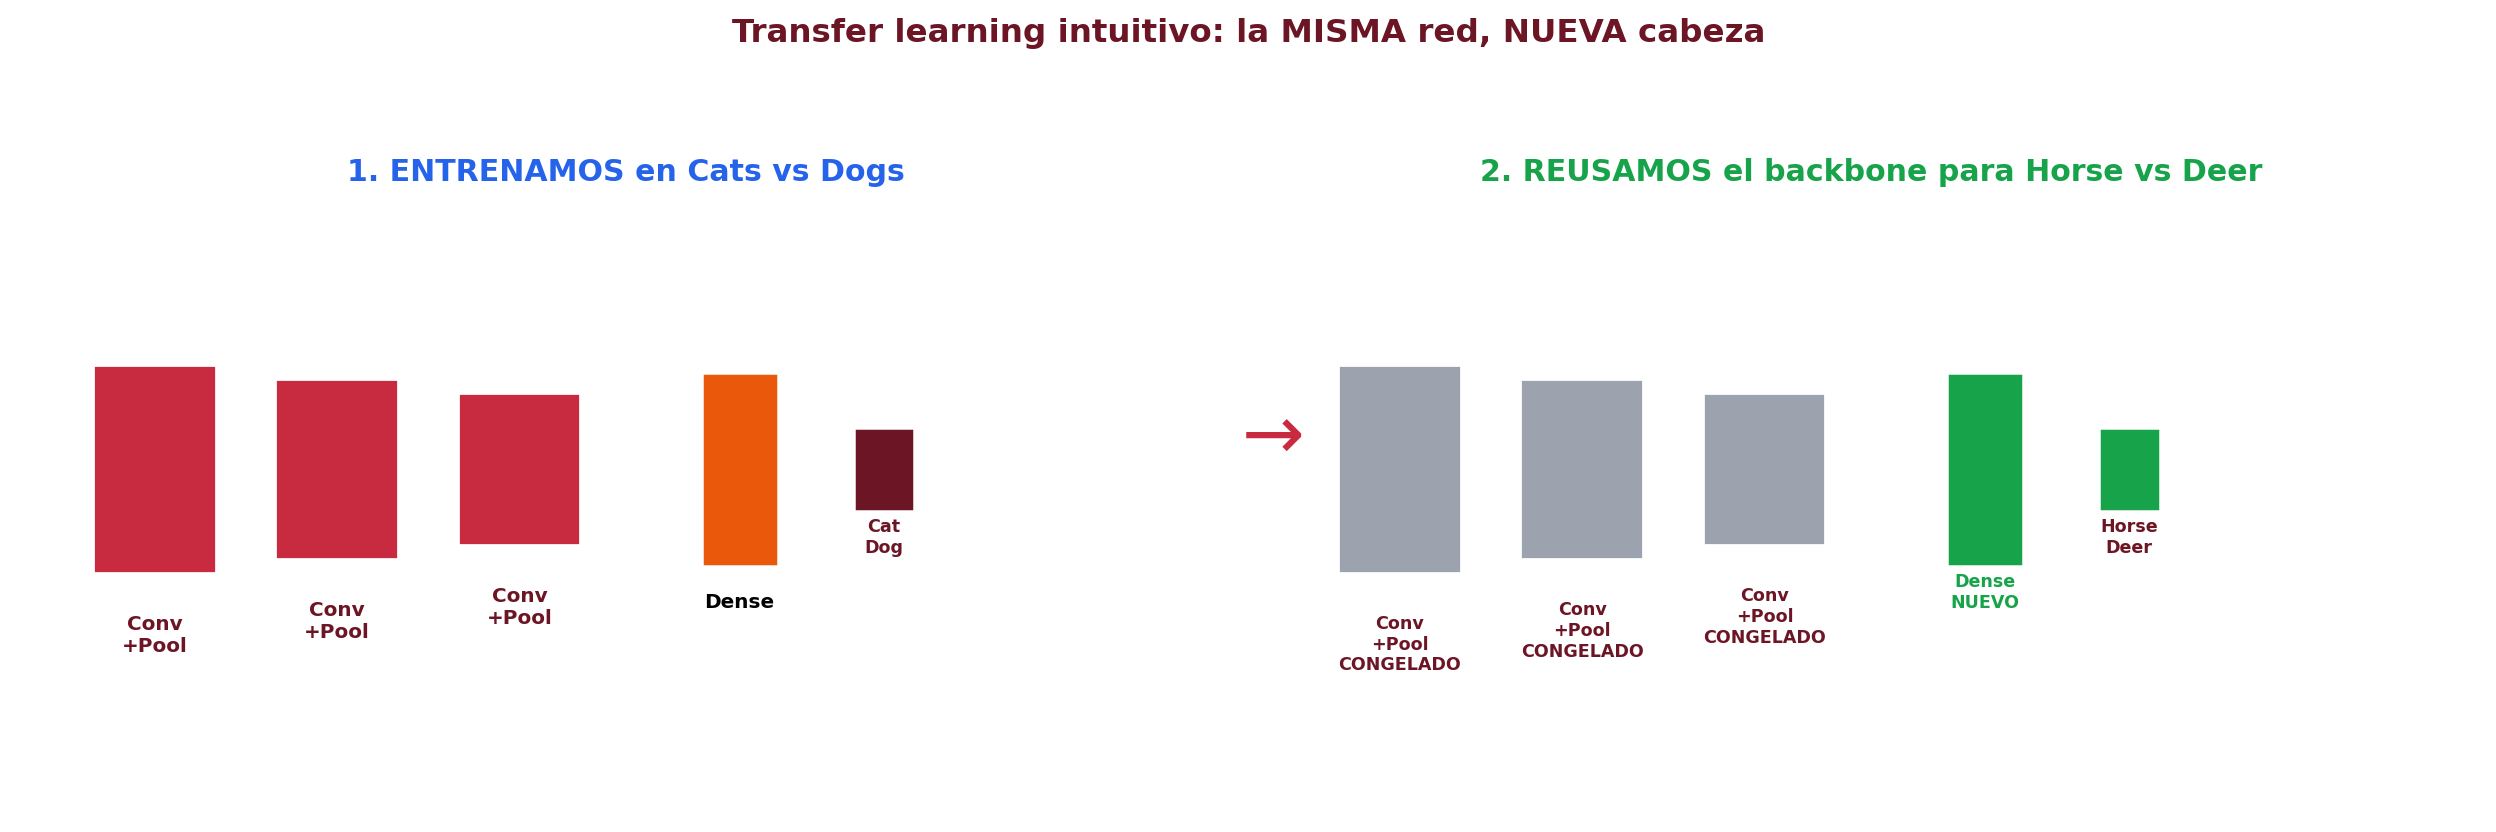
\includegraphics[width=0.95\textwidth]{../clase-24/fig_transfer_misma_red.png}
  \end{center}

  \vspace{4pt}
  {\scriptsize\color{textMuted}
    \faLightbulb\hspace{4pt} Para una nueva tarea: \emph{congelamos}
    los bloques convolucionales (no se reentrenan) y solo entrenamos
    una nueva cabeza Dense. Mucho menos datos y mucho menos c\'omputo.}
\end{frame}

\begin{frame}[shrink]{?`Por Qu\'e Funciona?}
  \vspace{8pt}
  {\footnotesize\color{arcaDark}\bfseries
    Las primeras capas convolucionales aprenden conceptos que son
    \textbf{los mismos en cualquier tarea de visi\'on}:}

  \vspace{14pt}
  {\footnotesize
  \begin{itemize}\setlength{\itemsep}{6pt}
    \item[{\color{arcaRed}\scriptsize\faArrowRight}]
      \textbf{Capas tempranas:} bordes, manchas, gradientes simples.
    \item[{\color{arcaRed}\scriptsize\faArrowRight}]
      \textbf{Capas medias:} texturas, esquinas, patrones repetitivos.
    \item[{\color{arcaRed}\scriptsize\faArrowRight}]
      \textbf{Capas tard\'ias:} partes (orejas, ojos, ruedas) y luego objetos.
    \item[{\color{codeGreen}\scriptsize\faArrowRight}]
      Solo las \emph{\'ultimas} capas son espec\'ificas de la tarea.
      Reusamos las primeras y reentrenamos las \'ultimas.
  \end{itemize}
  }
\end{frame}

\begin{frame}[shrink]{Modelos P\'ublicos: ?`Qu\'e Es ImageNet?}
  \vspace{4pt}
  {\footnotesize\color{arcaDark}\bfseries
    No es f\'acil entrenar una CNN buena: hace falta mucha data y
    mucha GPU. Por suerte otros ya lo hicieron --- en un dataset
    p\'ublico llamado \textbf{ImageNet}.}

  \vspace{14pt}
  \begin{center}
  \begin{tikzpicture}[
    fact/.style={rectangle, rounded corners=4pt, minimum width=2.7cm,
                 minimum height=2.6cm, align=center, text width=2.5cm,
                 inner sep=4pt, font=\scriptsize\color{white}},
  ]
    \node[fact, fill=codeBlue] (f1)
      {{\bfseries\large 1.4 millones}\\{\bfseries de im\'agenes}\\[4pt]
       Etiquetadas a mano por humanos};
    \node[fact, fill=codeOrange, right=6pt of f1] (f2)
      {{\bfseries\large 1\,000}\\{\bfseries categor\'ias}\\[4pt]
       Perros, autos, frutas, herramientas, animales\ldots};
    \node[fact, fill=codePurple, right=6pt of f2] (f3)
      {{\bfseries\large 224$\times$224}\\{\bfseries resoluci\'on}\\[4pt]
       Fotos reales del mundo (no MNIST)};
    \node[fact, fill=codeGreen, right=6pt of f3] (f4)
      {{\bfseries\large 2010--2017}\\{\bfseries Concurso}\\[4pt]
       Donde nacieron VGG, ResNet, Inception\ldots};
  \end{tikzpicture}
  \end{center}

  \vspace{8pt}
  {\scriptsize\color{textMuted}
    \faLightbulb\hspace{4pt} VGG16 ``vio'' 1.4M de fotos. Sus filtros
    aprendieron lo que es un \textbf{borde}, una \textbf{textura},
    un \textbf{ojo}. Sirven para casi cualquier problema de visi\'on.}
\end{frame}

\begin{frame}[shrink]{VGG16: La M\'as F\'acil de Leer}
  \vspace{4pt}
  {\footnotesize\color{arcaDark}\bfseries
    \textbf{VGG16} (Oxford, 2014) es una CNN que solo apila lo que
    ya conocemos: \texttt{Conv2D 3$\times$3} + \texttt{MaxPool} +
    \texttt{Dense}. \emph{Sin bloques especiales, sin atajos}.}

  \vspace{6pt}
  \begin{center}
    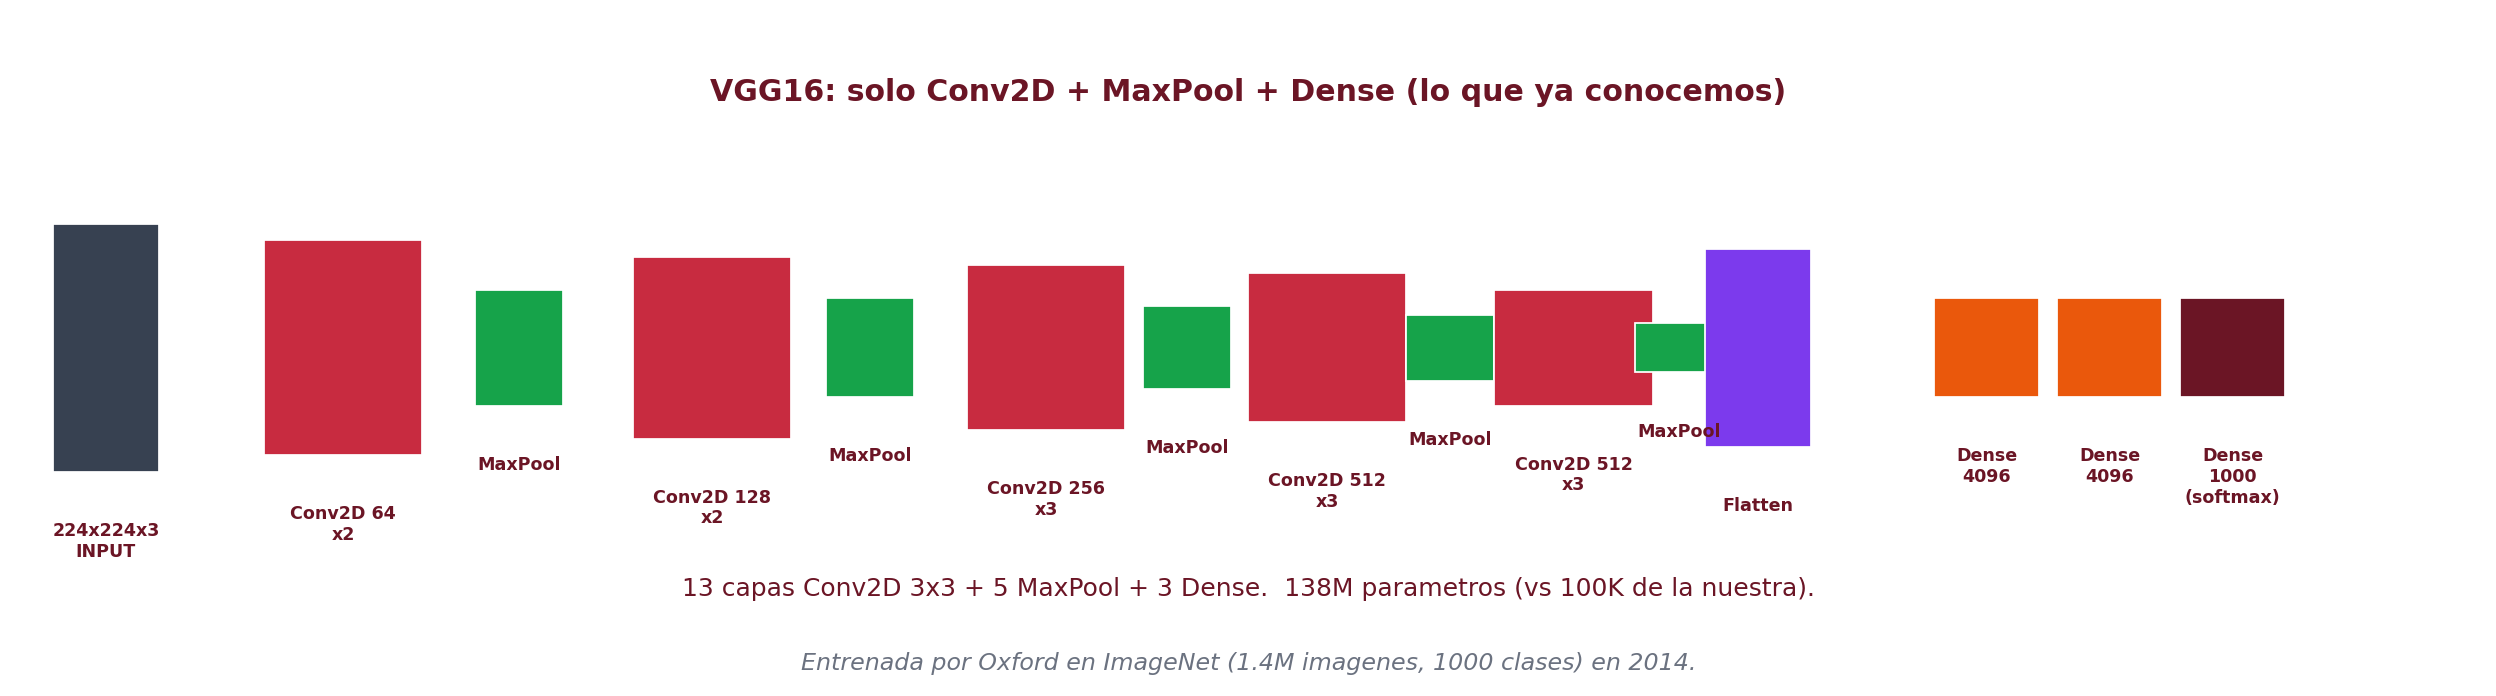
\includegraphics[width=0.97\textwidth]{../clase-24/fig_vgg16.png}
  \end{center}

  \vspace{2pt}
  {\scriptsize\color{textMuted}
    \faLightbulb\hspace{4pt} Esa simplicidad la hace
    \textbf{ideal para entender}. Existen modelos m\'as modernos
    (ResNet, EfficientNet) que son m\'as rapidos pero con bloques
    avanzados que veremos despu\'es.}
\end{frame}

\begin{frame}[shrink]{?`C\'omo Compara con Nuestra CNN?}
  \vspace{14pt}
  \begin{center}
  {\footnotesize
  \begin{tabular}{@{}>{\raggedright\arraybackslash}p{4cm}
                   >{\centering\arraybackslash}p{4cm}
                   >{\centering\arraybackslash}p{4cm}@{}}
    \toprule
    & \textbf{\color{arcaRed}Nuestra CNN}
    & \textbf{\color{codeGreen}VGG16} \\
    & {\scriptsize la que entrenamos hoy}
    & {\scriptsize la que reusamos} \\
    \midrule
    \rowcolor{arcaGray}
    Datos de entrenamiento
    & 4\,000 imagenes (cats vs dogs)
    & \textbf{1.4 millones} (ImageNet) \\
    Par\'ametros
    & $\sim$120 mil
    & \textbf{138 millones} \\
    \rowcolor{arcaGray}
    Capas convolucionales
    & 3 (Conv-Pool $\times$3)
    & \textbf{13} (5 bloques) \\
    Tiempo de entrenamiento (con GPU)
    & $\sim$2 minutos
    & \textbf{$\sim$3 semanas} (en 2014) \\
    \bottomrule
  \end{tabular}
  }
  \end{center}

  \vspace{12pt}
  \begin{tcolorbox}[colback=arcaRed!8, colframe=arcaRed, boxrule=0.5pt,
    arc=2pt, left=6pt, right=6pt, top=4pt, bottom=4pt]
    {\scriptsize\color{arcaDark}
    \faExclamationTriangle\hspace{4pt}\textbf{Imposible que nuestra CNN
    compita desde cero.} Por eso reusamos los pesos de VGG16: aunque
    nuestra tarea es distinta, \emph{los patrones visuales b\'asicos
    son los mismos}.}
  \end{tcolorbox}
\end{frame}

\begin{frame}[fragile,shrink]{Transfer Learning con VGG16 en C\'odigo}
  \vspace{-4pt}
  \begin{pyblock}
from tensorflow.keras.applications import VGG16

# 1. Cargar VGG16 SIN su cabeza, con pesos de ImageNet
base = VGG16(input_shape=(96,96,3), include_top=False, weights="imagenet")
base.trainable = False                 # congelar capas conv

# 2. Backbone congelado + cabeza nueva
modelo = Sequential([
    base,
    layers.Flatten(),
    layers.Dense(64, activation="relu"),
    layers.Dense(2, activation="softmax"),
])

# 3. Solo entrena el cabezal (pocos pesos, pocas epochs)
modelo.compile("adam", "sparse_categorical_crossentropy", ["accuracy"])
modelo.fit(X_train, y_train, epochs=5, validation_split=0.1)
  \end{pyblock}
\end{frame}

% =============================================================================
%  BLOQUE B: LIMITACIONES (copia de clase 24 / bloque 9)
% =============================================================================
\sectionframe{Limitaciones}{Cu\'ando NO entrenar una CNN desde cero}

\begin{frame}[shrink]{Cuatro Costos Reales de las CNN}
  \vspace{6pt}
  {\footnotesize
  \begin{tabular}{@{}p{2.6cm} p{10.0cm}@{}}
    \toprule
    \textbf{Costo} & \textbf{C\'omo se manifiesta} \\
    \midrule
    \rowcolor{arcaGray}
    \textbf{Datos}
    & Una CNN seria pide decenas de miles de im\'agenes etiquetadas.
      Si tienen 500, una CNN desde cero \emph{no funciona}. \\
    \textbf{C\'omputo}
    & GPU pr\'acticamente obligatoria. Sin ella, entrenar dataset grande
      toma horas o d\'ias. \\
    \rowcolor{arcaGray}
    \textbf{Hiperpar\'ametros}
    & Filtros, profundidad, learning rate, batch, dropout\ldots
      Mucho m\'as tuning que sklearn. \\
    \textbf{Interpretabilidad}
    & Dif\'icil decir ``por qu\'e'' la CNN predijo gato. T\'ecnicas
      como Grad-CAM ayudan, pero no como ``feature importance'' de RF. \\
    \bottomrule
  \end{tabular}
  }

  \vspace{14pt}
  \begin{tcolorbox}[colback=codeOrange!8, colframe=codeOrange, boxrule=0.5pt,
    arc=2pt, left=6pt, right=6pt, top=4pt, bottom=4pt]
    {\scriptsize\color{arcaDark}
    \faExclamationTriangle\hspace{4pt}\textbf{Antes de entrenar desde cero:}
    pregunten si pueden usar transfer learning. La respuesta casi siempre
    es s\'i.}
  \end{tcolorbox}
\end{frame}

\begin{frame}[shrink]{?`Cu\'ando Usar (y NO Usar) una CNN?}
  \vspace{4pt}
  \begin{center}
    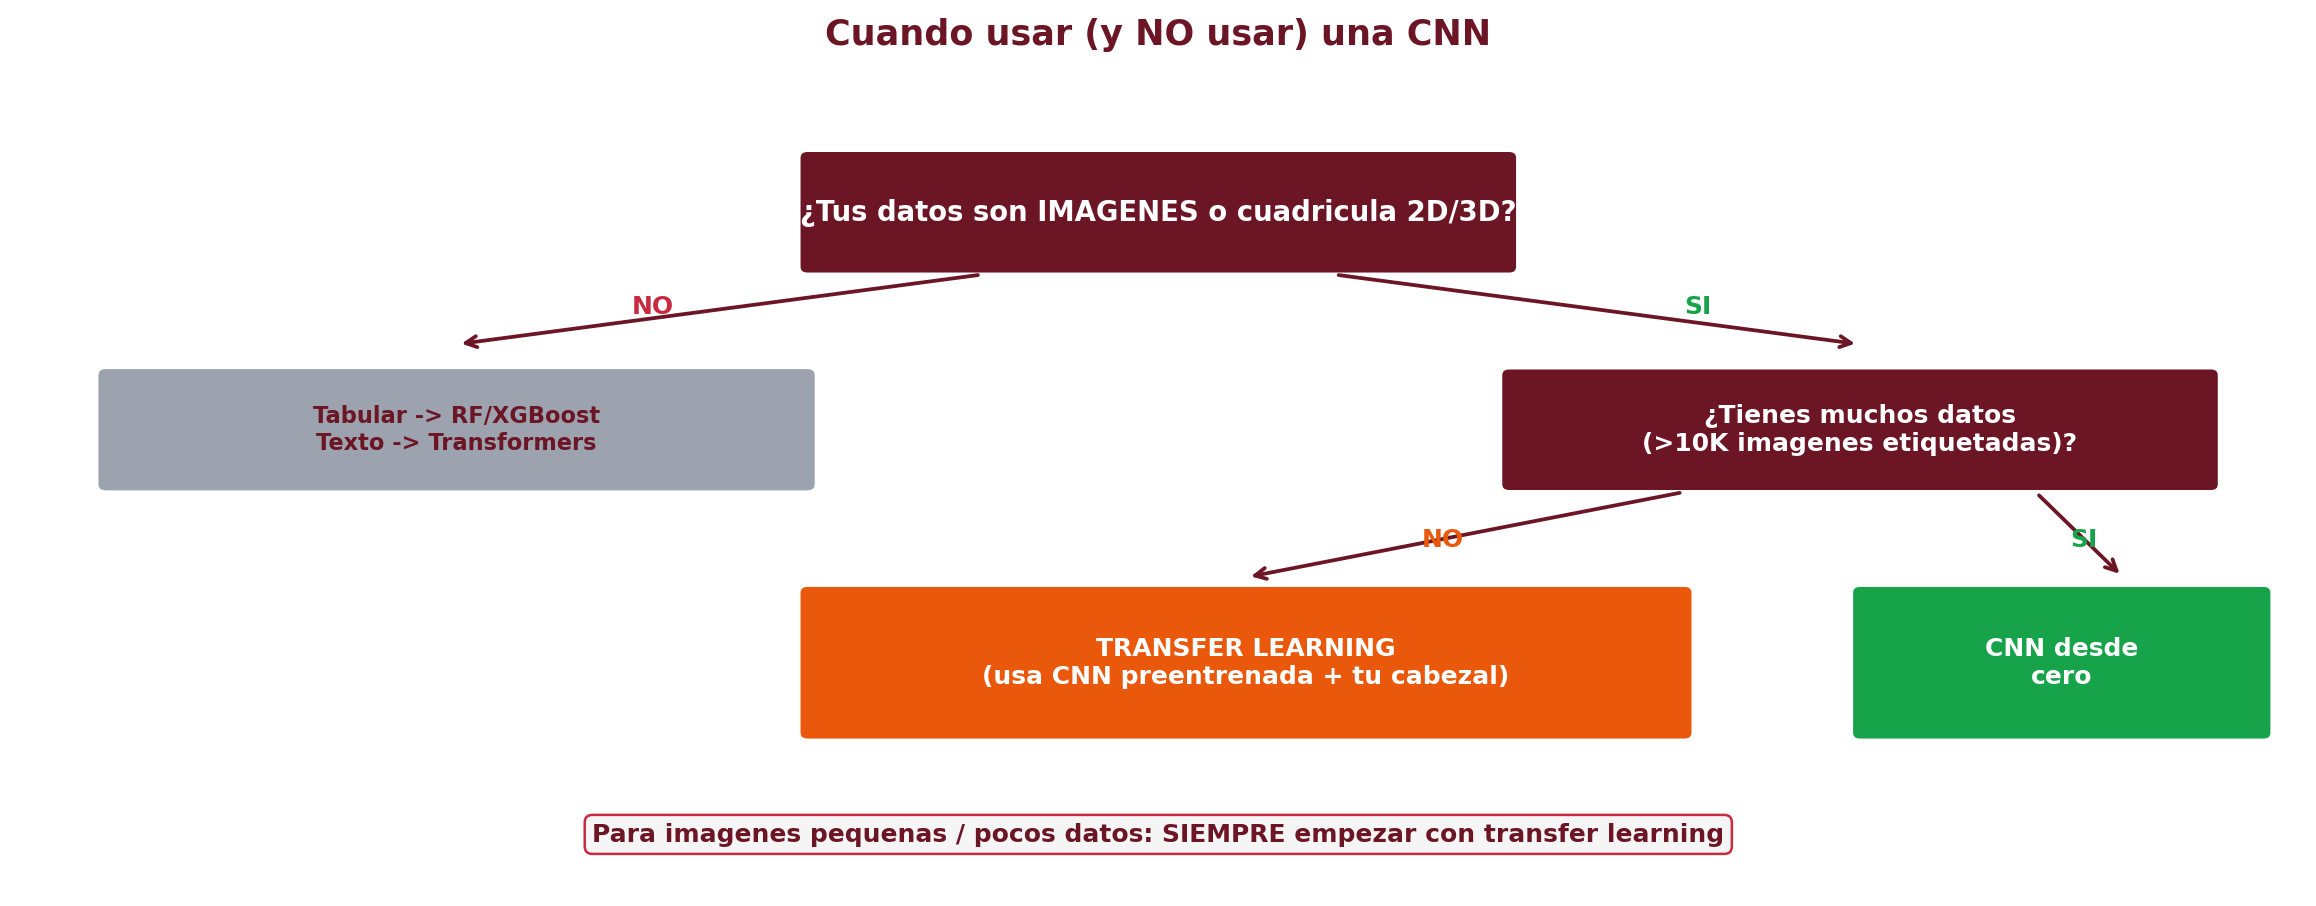
\includegraphics[width=0.92\textwidth]{../clase-24/fig_cuando_cnn.png}
  \end{center}

  \vspace{4pt}
  {\scriptsize
  \begin{itemize}\setlength{\itemsep}{2pt}
    \item[{\color{codeGreen}\scriptsize\faCheck}]
      \textbf{S\'i} CNN: im\'agenes, espectrogramas de audio,
      datos en cuadr\'icula 2D/3D.
    \item[{\color{arcaRed}\scriptsize\faTimes}]
      \textbf{No} CNN para tabular (RF/XGBoost), texto (Transformers),
      series temporales no espaciales.
  \end{itemize}
  }
\end{frame}

\begin{frame}[shrink]{Una Mirada al Futuro: Vision Transformers}
  \vspace{6pt}
  {\footnotesize\color{arcaDark}\bfseries
    Desde 2020 las \textbf{Vision Transformers (ViT)} compiten y
    a veces superan a las CNN. Importante saberlo --- pero
    nuestra base sigue siendo CNN.}

  \vspace{14pt}
  {\footnotesize
  \begin{itemize}\setlength{\itemsep}{6pt}
    \item[{\color{arcaRed}\scriptsize\faArrowRight}]
      \textbf{ViT} divide la imagen en parches 16$\times$16 y los trata
      como ``palabras'', con el mismo mecanismo que GPT.
    \item[{\color{arcaRed}\scriptsize\faArrowRight}]
      Modelos modernos (CLIP, DINOv2, Stable Diffusion) son a base de
      transformers / h\'ibridos.
    \item[{\color{codeGreen}\scriptsize\faArrowRight}]
      \textbf{Pero las CNN siguen siendo el caballo de batalla} cuando
      hay poca data, pocos recursos o restricciones de latencia
      (m\'oviles, IoT, l\'ineas de producci\'on).
  \end{itemize}
  }
\end{frame}

% =============================================================================
%  BLOQUE B': HIPERPARAMETROS QUE IMPORTAN (batch size + early stopping)
% =============================================================================
\sectionframe{Hiperpar\'ametros que Importan}{Batch size y early stopping en la pr\'actica}

\begin{frame}[shrink]{Batch Size: Cu\'antas Muestras Por Paso}
  \vspace{6pt}
  {\footnotesize\color{arcaDark}\bfseries
    \textbf{Batch size} = cu\'antas im\'agenes procesa el modelo
    \emph{antes} de actualizar sus pesos. Es de los hiperpar\'ametros
    que m\'as afectan c\'omo aprende.}

  \vspace{12pt}
  {\footnotesize
  \begin{tabular}{@{}p{2.4cm} p{4.5cm} p{5.0cm}@{}}
    \toprule
    \textbf{Batch size} & \textbf{Comportamiento} & \textbf{Cu\'ando usarlo} \\
    \midrule
    \rowcolor{arcaGray}
    \textbf{Peque\~no (8--32)}
    & Gradiente \emph{ruidoso}: cada paso es una estimaci\'on grosera.
      Generaliza mejor (act\'ua como regularizador).
    & Pocos datos, problemas dif\'iciles, modelos que sobreajustan. \\
    \textbf{Mediano (32--128)}
    & Equilibrio: gradiente estable, velocidad razonable.
    & \textbf{Default seguro.} Empezar aqu\'i casi siempre. \\
    \rowcolor{arcaGray}
    \textbf{Grande (256+)}
    & Gradiente muy estable, entrenamiento r\'apido,
      pero \emph{tiende a memorizar}. Necesita m\'as regularizaci\'on.
    & Datasets enormes, GPUs grandes, fine-tuning corto. \\
    \bottomrule
  \end{tabular}
  }

  \vspace{10pt}
  \begin{tcolorbox}[colback=codeGreen!8, colframe=codeGreen, boxrule=0.5pt,
    arc=2pt, left=6pt, right=6pt, top=4pt, bottom=4pt]
    {\scriptsize\color{arcaDark}
    \faKey\hspace{4pt}\textbf{Regla pr\'actica:} arrancar con
    \texttt{batch\_size=32} (o 64 si tienes GPU). Si overfittea,
    bajarlo. Si va lent\'isimo, subirlo.}
  \end{tcolorbox}
\end{frame}

\begin{frame}[fragile,shrink]{Early Stopping: Parar a Tiempo}
  \vspace{6pt}
  {\footnotesize\color{arcaDark}\bfseries
    Entrenar de m\'as no mejora --- empeora. La curva t\'ipica:
    \texttt{val\_loss} baja, toca su m\'inimo, y empieza a \textbf{subir}.
    Eso es \emph{overfitting} en acci\'on.}

  \vspace{8pt}
  \begin{center}
  \begin{tikzpicture}[scale=0.85]
    \draw[->, gray] (0,0) -- (8.5,0) node[right, font=\scriptsize] {epoch};
    \draw[->, gray] (0,0) -- (0,3.2) node[above, font=\scriptsize] {loss};
    % train loss: monotonically decreasing
    \draw[arcaRed, thick] plot[smooth] coordinates
      {(0,3) (1,2.2) (2,1.6) (3,1.15) (4,0.8) (5,0.55) (6,0.38) (7,0.25) (8,0.18)};
    \node[arcaRed, font=\scriptsize\bfseries] at (8.4,0.18) {train};
    % val loss: U-shaped, minimum around epoch 4
    \draw[codeBlue, thick] plot[smooth] coordinates
      {(0,2.8) (1,2.0) (2,1.5) (3,1.2) (4,1.05) (5,1.15) (6,1.45) (7,1.85) (8,2.3)};
    \node[codeBlue, font=\scriptsize\bfseries] at (8.4,2.3) {val};
    % vertical line at best epoch
    \draw[codeGreen, thick, dashed] (4,0) -- (4,1.05);
    \node[codeGreen, font=\scriptsize\bfseries, align=center] at (4,3.05)
      {mejor\\ \'epoca};
    % shaded "stopped" region
    \fill[arcaRed, opacity=0.08] (4,0) rectangle (8,3);
    \node[arcaRed, font=\scriptsize, align=center] at (6,2.7)
      {entrenando de m\'as\\(overfitting)};
  \end{tikzpicture}
  \end{center}

  \vspace{4pt}
  \begin{pyblock}
from tensorflow.keras.callbacks import EarlyStopping

es = EarlyStopping(monitor="val_loss",
                   patience=3,                 # 3 epochs sin mejorar -> parar
                   restore_best_weights=True)  # vuelve a los pesos de la mejor epoca

modelo.fit(X_tr, y_tr, epochs=50, validation_split=0.1, callbacks=[es])
  \end{pyblock}

  \vspace{4pt}
  {\scriptsize\color{textMuted}
    \faLightbulb\hspace{4pt} \textbf{\texttt{restore\_best\_weights=True}}
    es la l\'inea m\'as importante: al parar, no te quedas con los
    pesos de la \'ultima \'epoca (que ya overfittea), sino con los de
    la mejor val\_loss vista.}
\end{frame}

% =============================================================================
%  BLOQUE C: CONSTRUIR DATASET (copia de clase 24 / bloque 10)
% =============================================================================
\sectionframe{Construir tu propio dataset}{Lo que m\'as importa --- y lo que m\'as cuesta}

\begin{frame}[shrink]{Tu Turno: Resolver un Problema Real}
  \vspace{6pt}
  {\footnotesize\color{arcaDark}\bfseries
    Hasta ahora usamos datasets que alguien m\'as recolect\'o. Ahora
    \textbf{ustedes} construyen el dataset \textbf{y} el clasificador.
    Para un problema que tenga sentido para Arca o para su \'area.}

  \vspace{14pt}
  {\footnotesize\color{arcaDark}\bfseries Ideas de problemas binarios (eligen uno o proponen otro):}

  \vspace{6pt}
  {\footnotesize
  \begin{itemize}\setlength{\itemsep}{4pt}
    \item[{\color{arcaRed}\scriptsize\faArrowRight}]
      \textbf{Anaquel lleno vs anaquel vac\'io} ---
      \emph{caso real de retail.} Detectar autom\'aticamente cu\'ando una g\'ondola
      necesita reposici\'on.
    \item[{\color{arcaRed}\scriptsize\faArrowRight}]
      \textbf{Lata vs botella PET} --- formato de empaque (f\'acil de buscar im\'agenes).
    \item[{\color{arcaRed}\scriptsize\faArrowRight}]
      \textbf{Producto Arca vs competencia} (Coca vs Inca, etc.).
    \item[{\color{arcaRed}\scriptsize\faArrowRight}]
      \textbf{Etiqueta legible vs da\~nada} --- control de calidad.
    \item[{\color{arcaRed}\scriptsize\faArrowRight}]
      \textbf{Camion cargado vs vac\'io} --- log\'istica.
    \item[{\color{codeGreen}\scriptsize\faArrowRight}]
      \textbf{Tu propuesta:} cualquier problema relevante a tu trabajo.
  \end{itemize}
  }
\end{frame}

\begin{frame}[shrink]{Construir un Buen Dataset: 5 Reglas de Oro}
  \vspace{6pt}
  {\footnotesize
  \begin{tabular}{@{}p{3.5cm} p{9.0cm}@{}}
    \toprule
    \textbf{Regla} & \textbf{Por qu\'e importa} \\
    \midrule
    \rowcolor{arcaGray}
    \textbf{1. Balance de clases}
    & Similar n\'umero de fotos por clase. Si tienes 200 ``llenas''
      y 20 ``vac\'ias'', el modelo aprende a decir ``lleno'' siempre. \\
    \textbf{2. Diversidad}
    & Distintos \'angulos, luces, distancias, fondos. Si todas las
      ``vac\'ias'' son del mismo Oxxo, el modelo aprende el \emph{Oxxo},
      no el ``vac\'io''. \\
    \rowcolor{arcaGray}
    \textbf{3. Train/test disjuntos}
    & Nunca dejar la misma foto (ni casi-duplicados) en train y test.
      Si no, el accuracy es una mentira. \\
    \textbf{4. Etiquetado consistente}
    & Las clases deben ser inequ\'ivocas. ?`Qu\'e es ``medio lleno''?
      Definir reglas \emph{antes} de etiquetar. \\
    \rowcolor{arcaGray}
    \textbf{5. Calidad $\,>\,$ cantidad}
    & 200 fotos buenas y diversas $>$ 1\,000 fotos repetitivas.
      Mejor menos pero limpio. \\
    \bottomrule
  \end{tabular}
  }
\end{frame}

\begin{frame}[shrink]{Errores Comunes (No Caigan en Estos)}
  \vspace{6pt}
  {\footnotesize
  \begin{tabular}{@{}p{4.5cm} p{8.0cm}@{}}
    \toprule
    \textbf{Error} & \textbf{Qu\'e pasa} \\
    \midrule
    \rowcolor{arcaRed!8}
    \textbf{Sesgo de fuente}
    & Todas las ``llenas'' de Google Images, todas las ``vac\'ias'' de
      Pinterest. El modelo aprende \emph{el sitio web}, no el problema. \\
    \textbf{Resoluci\'on inconsistente}
    & Mezclar fotos 4K con fotos 100$\times$100. Resize a un tama\~no
      \'unico (96$\times$96 o 224$\times$224) ANTES de entrenar. \\
    \rowcolor{arcaRed!8}
    \textbf{Im\'agenes ambiguas}
    & ``Anaquel medio lleno'' --- ?`d\'onde va? Decidir reglas
      previamente o agregar una clase ``intermedia''. \\
    \textbf{Test set contaminado}
    & Agregar fotos del mismo evento (mismo d\'ia, misma tienda) en
      train y test. Test debe venir de \emph{otra} tienda u otro d\'ia. \\
    \rowcolor{arcaRed!8}
    \textbf{Ignorar la distribuci\'on de producci\'on}
    & Si el modelo va a usarse de noche con luz tenue, no entrenar
      solo con fotos de d\'ia. El dataset debe parecerse a la realidad
      donde ser\'a desplegado. \\
    \bottomrule
  \end{tabular}
  }
\end{frame}

\begin{frame}[shrink]{D\'onde Conseguir Im\'agenes}
  \vspace{6pt}
  {\footnotesize
  \begin{tabular}{@{}p{3.8cm} p{8.5cm}@{}}
    \toprule
    \textbf{Fuente} & \textbf{Cu\'ando usarla} \\
    \midrule
    \rowcolor{arcaGray}
    \textbf{Google Images / Bing}
    & R\'apido, mucha variedad, pero cuidado con sesgos.
      M\'as f\'acil para problemas gen\'ericos (perro, gato, lata). \\
    \textbf{Tu propio celular}
    & La mejor opci\'on para problemas espec\'ificos de tu trabajo.
      Salir a tomar fotos en distintas tiendas / l\'ineas. \\
    \rowcolor{arcaGray}
    \textbf{Webcam con Gradio}
    & Captar fotos en vivo desde el notebook. Ideal para
      datasets peque\~nos. \\
    \textbf{Datasets p\'ublicos}
    & \texttt{kaggle.com}, \texttt{huggingface.co/datasets},
      \texttt{Open Images}. Buscar el problema antes de empezar de cero. \\
    \rowcolor{arcaGray}
    \textbf{Web scraping}
    & Cuando hay un sitio espec\'ifico (catalogo de productos).
      Verificar t\'erminos de uso. \\
    \bottomrule
  \end{tabular}
  }

  \vspace{8pt}
  \begin{tcolorbox}[colback=codeGreen!8, colframe=codeGreen, boxrule=0.5pt,
    arc=2pt, left=6pt, right=6pt, top=4pt, bottom=4pt]
    {\scriptsize\color{arcaDark}
    \faKey\hspace{4pt}\textbf{Para empezar:} 50--100 fotos por clase
    desde Google Images. Si funciona, ampl\'iar con fotos propias.}
  \end{tcolorbox}
\end{frame}

\begin{frame}[shrink]{Plan de Trabajo (Para Esta Semana)}
  \vspace{6pt}
  {\footnotesize\color{arcaDark}\bfseries
    Lo construimos paso a paso en el notebook.
    Entregable: link p\'ublico de Gradio + screenshot de m\'etricas.}

  \vspace{12pt}
  \begin{center}
  \begin{tikzpicture}[
    pstep/.style={rectangle, rounded corners=4pt, minimum width=2.4cm,
                 minimum height=1.7cm, align=center, text width=2.2cm,
                 inner sep=4pt, font=\scriptsize\color{white}\bfseries},
  ]
    \node[pstep, fill=codeBlue]   (s1)
      {1. ELEGIR\\problema\\\scriptsize\mdseries y 2--3 clases};
    \node[pstep, fill=codeOrange, right=4pt of s1] (s2)
      {2. RECOLECTAR\\50--100 por clase\\\scriptsize\mdseries diverso};
    \node[pstep, fill=codePurple, right=4pt of s2] (s3)
      {3. ETIQUETAR\\y limpiar\\\scriptsize\mdseries reglas claras};
    \node[pstep, fill=arcaRed, right=4pt of s3]   (s4)
      {4. ENTRENAR\\transfer learning\\\scriptsize\mdseries VGG16 + cabeza};
    \node[pstep, fill=codeGreen, right=4pt of s4] (s5)
      {5. EVALUAR\\confusion matrix\\\scriptsize\mdseries no solo accuracy};
    \node[pstep, fill=arcaDark, right=4pt of s5]  (s6)
      {6. DESPLEGAR\\Gradio app\\\scriptsize\mdseries link p\'ublico};

    \draw[->, line width=1pt, arcaDark] (s1) -- (s2);
    \draw[->, line width=1pt, arcaDark] (s2) -- (s3);
    \draw[->, line width=1pt, arcaDark] (s3) -- (s4);
    \draw[->, line width=1pt, arcaDark] (s4) -- (s5);
    \draw[->, line width=1pt, arcaDark] (s5) -- (s6);
  \end{tikzpicture}
  \end{center}

  \vspace{8pt}
  {\scriptsize\color{textMuted}
    \faLightbulb\hspace{4pt} Este es el flujo est\'andar para
    \emph{cualquier} clasificador de im\'agenes. En adelante asumimos
    que ya saben armarlo.}
\end{frame}

% =============================================================================
%  BLOQUE D: TAREAS DE VISION POR COMPUTADORA
% =============================================================================
\sectionframe{Tareas de Visi\'on por Computadora}{Cinco maneras distintas de ``ver''}

\begin{frame}[shrink]{Las 5 Tareas Principales}
  \vspace{8pt}
  {\footnotesize
  \begin{tabular}{@{}p{3.0cm} p{4.5cm} p{5.0cm}@{}}
    \toprule
    \textbf{Tarea} & \textbf{Salida} & \textbf{Pregunta que responde} \\
    \midrule
    \rowcolor{arcaGray}
    \textbf{Clasificaci\'on}
    & 1 etiqueta por imagen
    & ?`Qu\'e hay en la imagen? \\
    \textbf{Detecci\'on}
    & N bounding boxes + clase
    & ?`Qu\'e hay y \emph{d\'onde}? \\
    \rowcolor{arcaGray}
    \textbf{Segmentaci\'on}
    & M\'ascara por pixel
    & ?`Qu\'e \emph{pixeles} son cada cosa? \\
    \textbf{Pose / keypoints}
    & Puntos clave conectados
    & ?`D\'onde est\'an las articulaciones? \\
    \rowcolor{arcaGray}
    \textbf{OCR}
    & Texto extra\'ido
    & ?`Qu\'e \emph{dice} la imagen? \\
    \bottomrule
  \end{tabular}
  }

  \vspace{14pt}
  \begin{tcolorbox}[colback=codeGreen!8, colframe=codeGreen, boxrule=0.5pt,
    arc=2pt, left=6pt, right=6pt, top=4pt, bottom=4pt]
    {\scriptsize\color{arcaDark}
    \faKey\hspace{4pt}\textbf{Hoy:} miramos cada una con un ejemplo,
    luego nos enfocamos en \textbf{detecci\'on}.}
  \end{tcolorbox}
\end{frame}

\begin{frame}[shrink]{1. Clasificaci\'on}
  \vspace{4pt}
  \begin{center}
    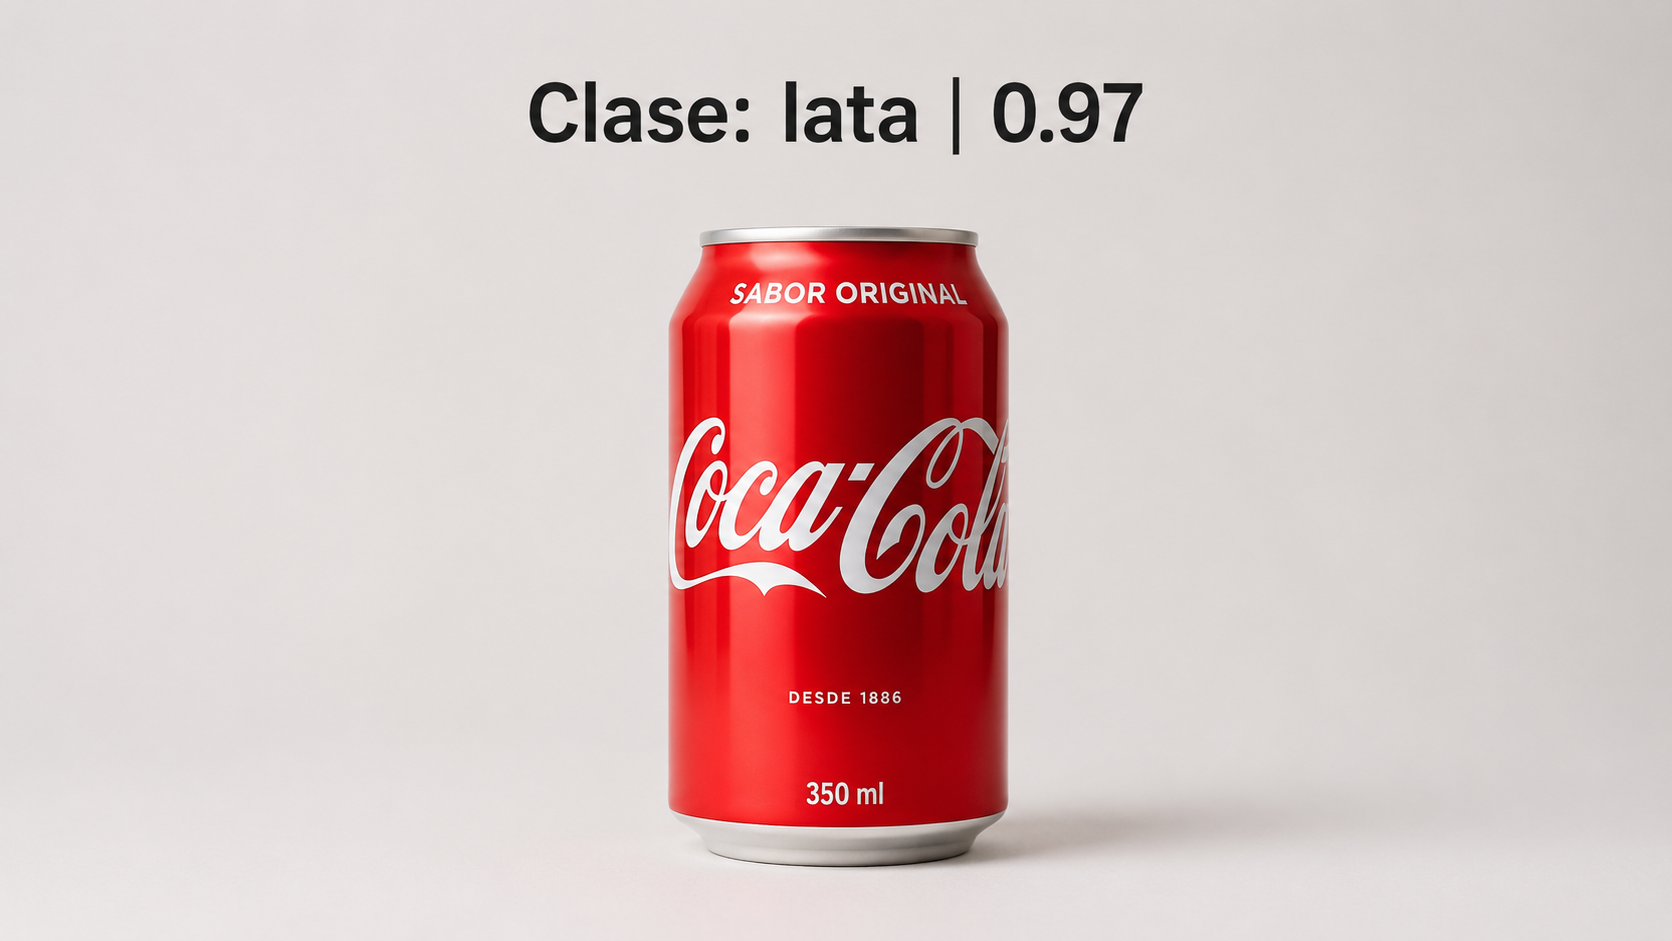
\includegraphics[width=0.55\textwidth]{fig_task_classification.png}
  \end{center}

  \vspace{4pt}
  {\footnotesize
  \begin{itemize}\setlength{\itemsep}{2pt}
    \item[{\color{arcaRed}\scriptsize\faArrowRight}]
      \textbf{Salida:} una etiqueta y su confianza (``lata'' 0.97).
    \item[{\color{arcaRed}\scriptsize\faArrowRight}]
      Asume que hay \textbf{un objeto principal} en la imagen.
    \item[{\color{arcaRed}\scriptsize\faArrowRight}]
      Lo que hicimos en clases 22--24: MNIST, Fashion MNIST, Cats vs Dogs, Coca vs Pepsi.
  \end{itemize}
  }
\end{frame}

\begin{frame}[shrink]{2. Detecci\'on}
  \vspace{4pt}
  \begin{center}
    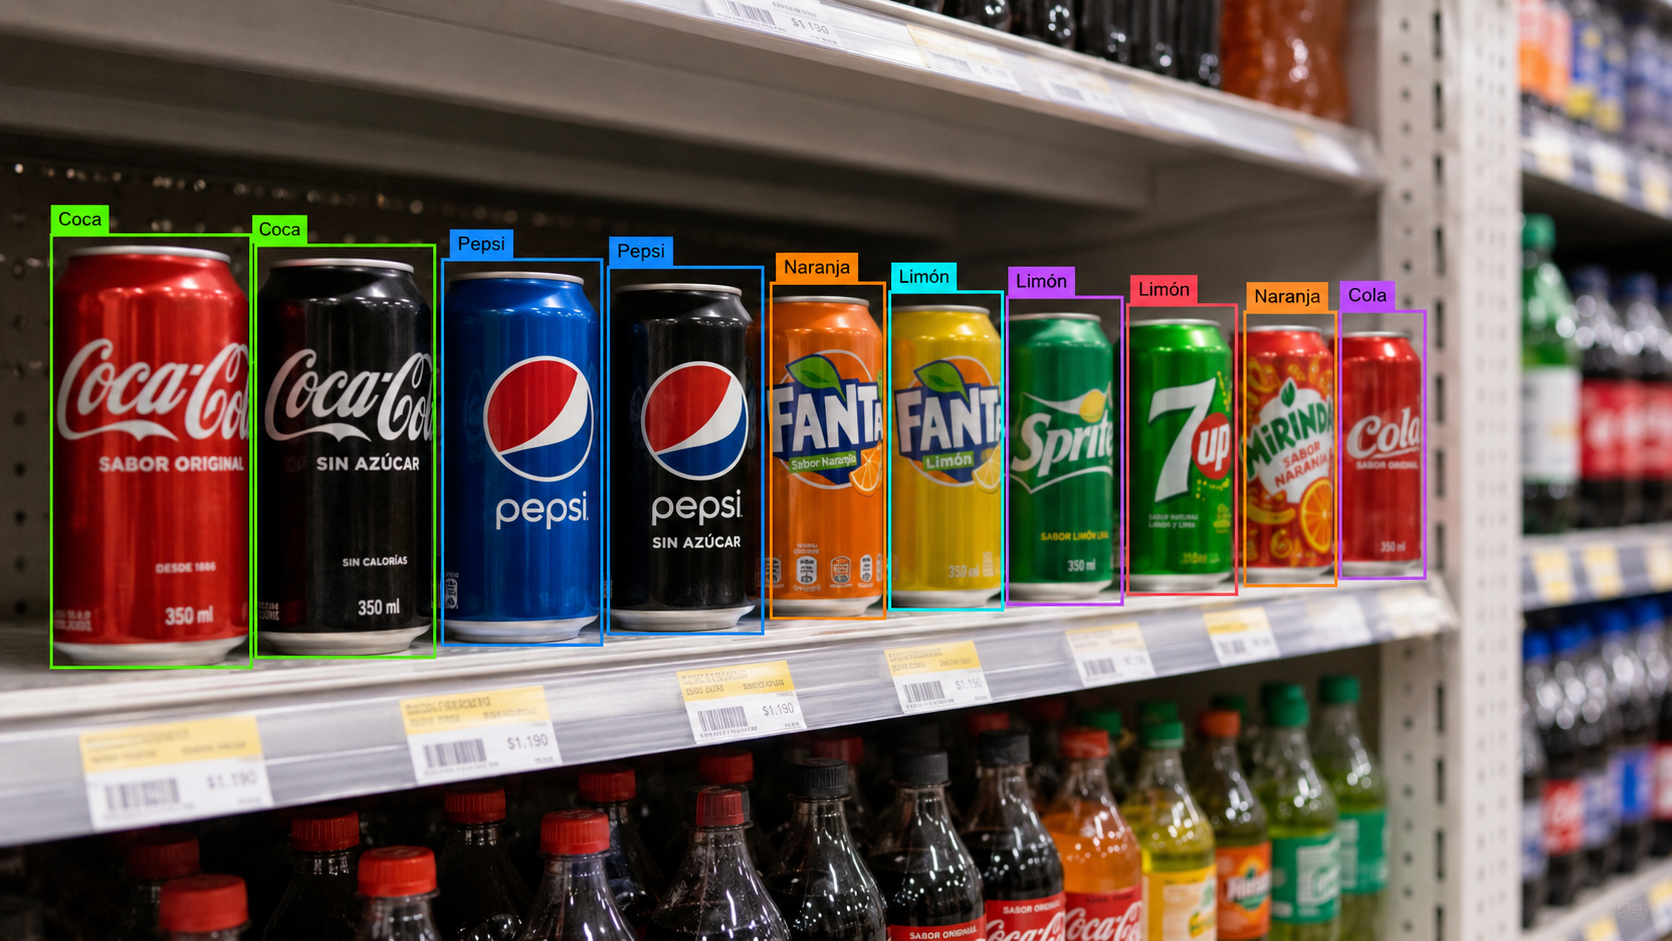
\includegraphics[width=0.78\textwidth]{fig_task_detection.png}
  \end{center}

  \vspace{4pt}
  {\footnotesize
  \begin{itemize}\setlength{\itemsep}{2pt}
    \item[{\color{arcaRed}\scriptsize\faArrowRight}]
      \textbf{Salida:} lista de bboxes \texttt{(x, y, w, h, clase)}, una por objeto.
    \item[{\color{arcaRed}\scriptsize\faArrowRight}]
      Maneja \textbf{m\'ultiples objetos} simult\'aneos en una sola imagen.
  \end{itemize}
  }
\end{frame}

\begin{frame}[shrink]{3. Segmentaci\'on}
  \vspace{4pt}
  \begin{center}
    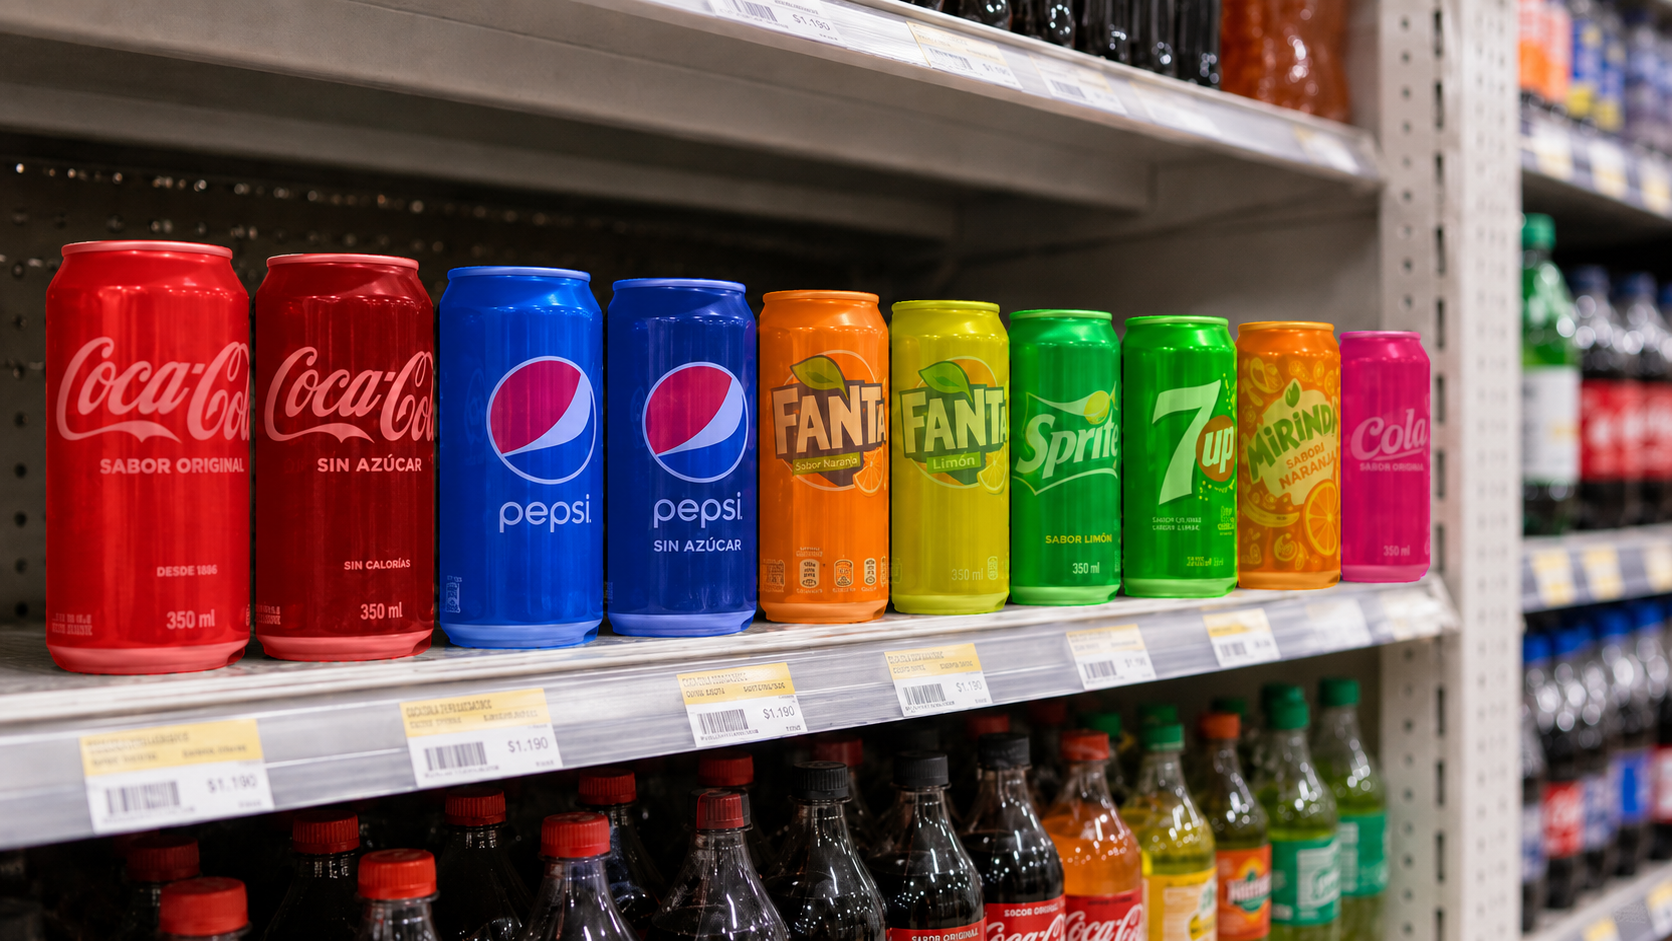
\includegraphics[width=0.78\textwidth]{fig_task_segmentation.png}
  \end{center}

  \vspace{4pt}
  {\footnotesize
  \begin{itemize}\setlength{\itemsep}{2pt}
    \item[{\color{arcaRed}\scriptsize\faArrowRight}]
      \textbf{Salida:} m\'ascara por \emph{pixel} (cada pixel etiquetado).
    \item[{\color{arcaRed}\scriptsize\faArrowRight}]
      M\'as costoso de etiquetar y entrenar, pero precisi\'on al pixel.
    \item[{\color{arcaRed}\scriptsize\faArrowRight}]
      Casos: medicina (delimitar tumor), agricultura (\'area cultivada).
  \end{itemize}
  }
\end{frame}

\begin{frame}[shrink]{4. Pose / Keypoints}
  \vspace{4pt}
  \begin{center}
    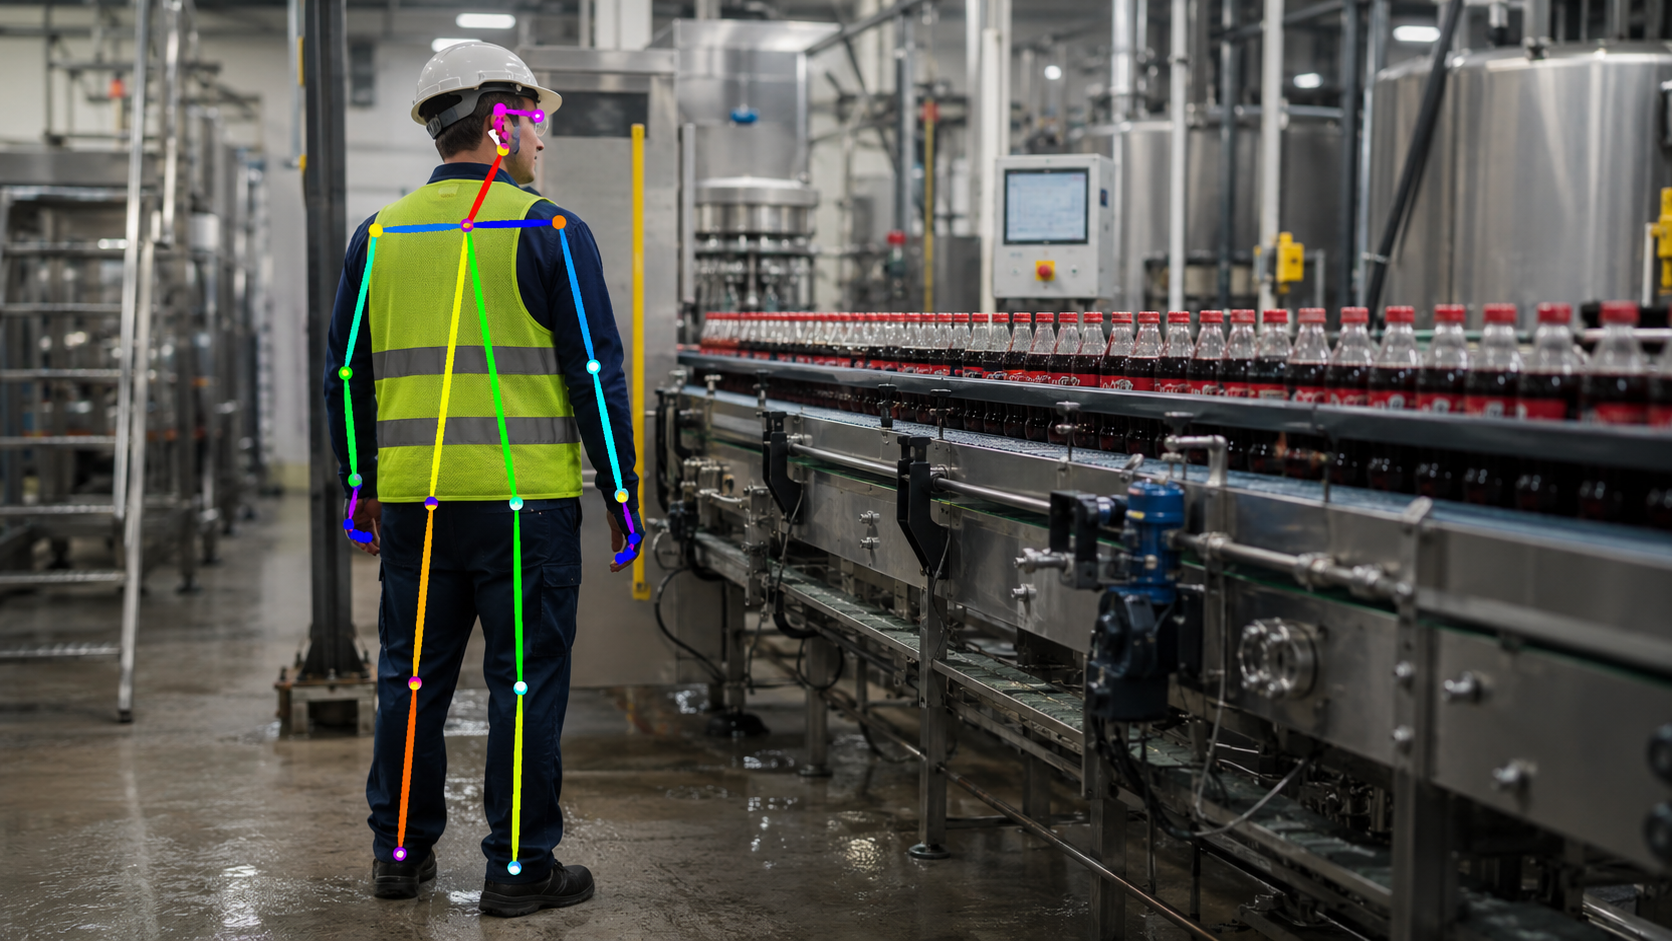
\includegraphics[width=0.78\textwidth]{fig_task_pose.png}
  \end{center}

  \vspace{4pt}
  {\footnotesize
  \begin{itemize}\setlength{\itemsep}{2pt}
    \item[{\color{arcaRed}\scriptsize\faArrowRight}]
      \textbf{Salida:} puntos clave (articulaciones) conectados.
    \item[{\color{arcaRed}\scriptsize\faArrowRight}]
      Casos: an\'alisis deportivo, ergonom\'ia, vigilancia de movimientos.
  \end{itemize}
  }
\end{frame}

\begin{frame}[shrink]{5. OCR (lectura de texto)}
  \vspace{4pt}
  \begin{center}
    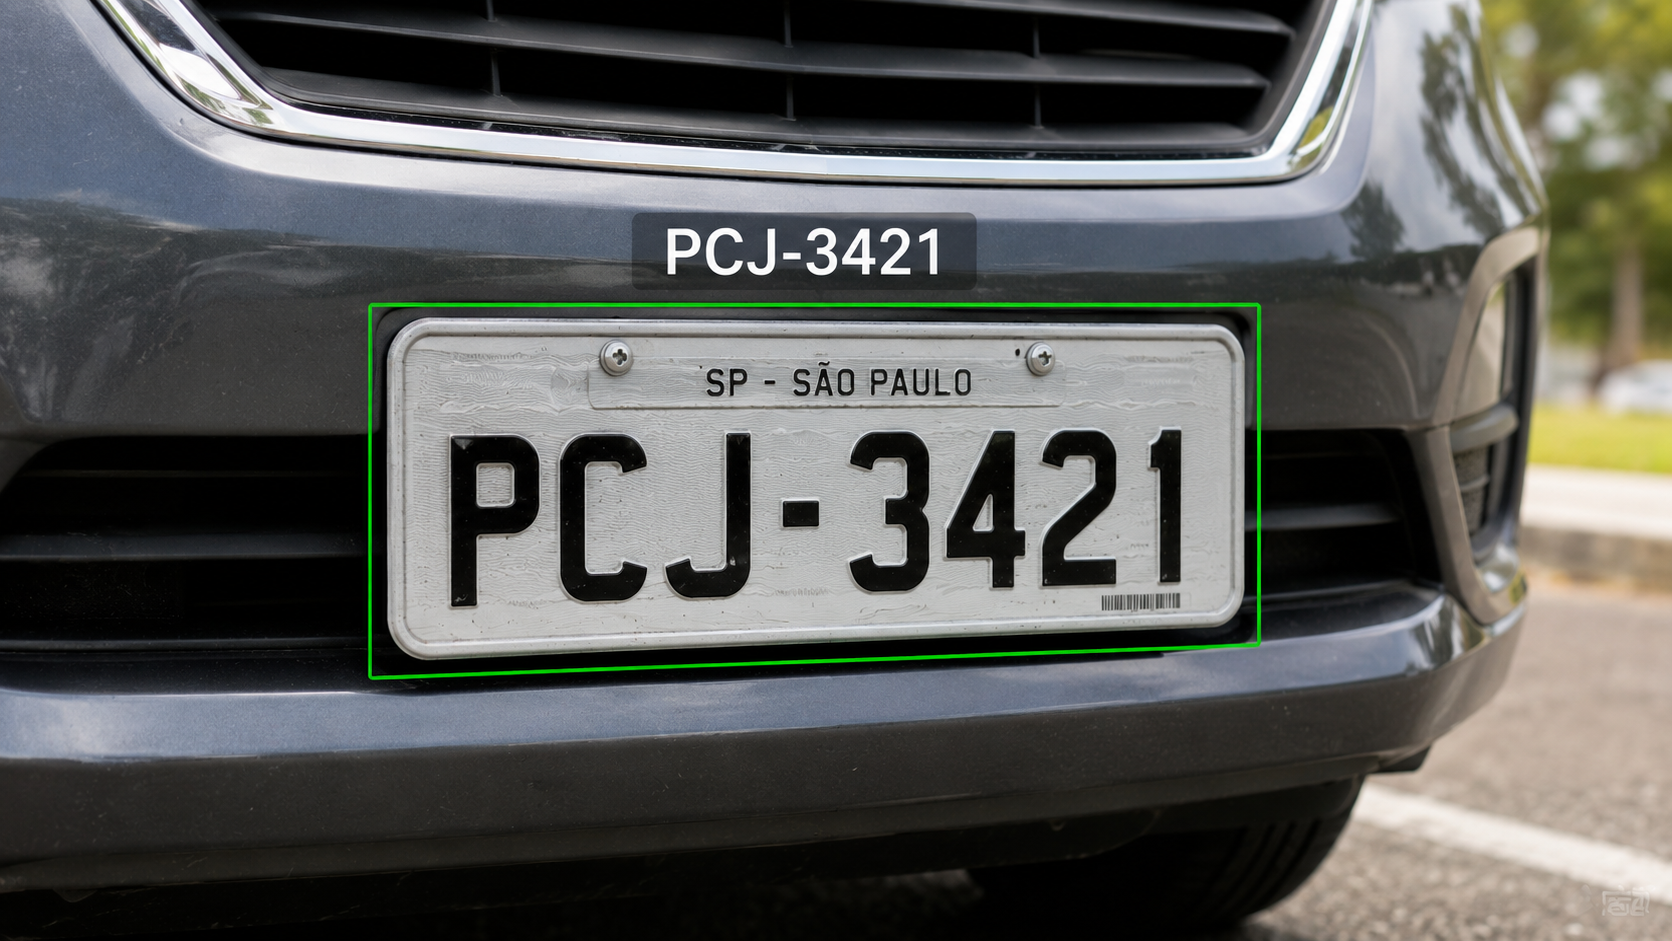
\includegraphics[width=0.78\textwidth]{fig_task_ocr.png}
  \end{center}

  \vspace{4pt}
  {\footnotesize
  \begin{itemize}\setlength{\itemsep}{2pt}
    \item[{\color{arcaRed}\scriptsize\faArrowRight}]
      \textbf{Salida:} la cadena de texto extra\'ida.
    \item[{\color{arcaRed}\scriptsize\faArrowRight}]
      Casos: lectura de placas, fechas de vencimiento, lotes, recibos.
    \item[{\color{codeGreen}\scriptsize\faArrowRight}]
      Suele combinarse con detecci\'on: detectar el rect\'angulo $\to$ leer el texto adentro.
  \end{itemize}
  }
\end{frame}

\begin{frame}[shrink]{?`Cu\'al Tarea Para Cu\'al Problema?}
  \vspace{8pt}
  {\footnotesize
  \begin{tabular}{@{}p{6.0cm} p{6.5cm}@{}}
    \toprule
    \textbf{Si tu pregunta es\ldots} & \textbf{La tarea es\ldots} \\
    \midrule
    \rowcolor{arcaGray}
    ?`Esta lata est\'a defectuosa? (1 producto por foto)
    & Clasificaci\'on \\
    ?`Cu\'antas latas hay en la g\'ondola y de qu\'e marca?
    & Detecci\'on \\
    \rowcolor{arcaGray}
    ?`Qu\'e \'area de la cinta transportadora ocupa el producto?
    & Segmentaci\'on \\
    ?`El operario tiene la mano cerca de zona peligrosa?
    & Pose / keypoints \\
    \rowcolor{arcaGray}
    ?`Cu\'al es el c\'odigo de lote impreso en esta caja?
    & OCR \\
    ?`Qu\'e dice la placa del cami\'on que ingresa?
    & \textbf{Detecci\'on + OCR (cascada)} \\
    \bottomrule
  \end{tabular}
  }

  \vspace{14pt}
  \begin{tcolorbox}[colback=arcaGray, colframe=arcaRed, boxrule=0.5pt,
    arc=2pt, left=6pt, right=6pt, top=4pt, bottom=4pt]
    {\scriptsize\color{arcaDark}
    \faKey\hspace{4pt}\textbf{Hoy nos enfocamos en detecci\'on}: c\'omo
    salir de ``una respuesta por imagen'' a ``N respuestas con su ubicaci\'on''.}
  \end{tcolorbox}
\end{frame}

% =============================================================================
%  BLOQUE E: BOUNDING BOXES + IoU
% =============================================================================
\sectionframe{Bounding Boxes e IoU}{La gram\'atica de la detecci\'on}

\begin{frame}[shrink]{Anatom\'ia de un Bounding Box}
  \vspace{4pt}
  \begin{center}
    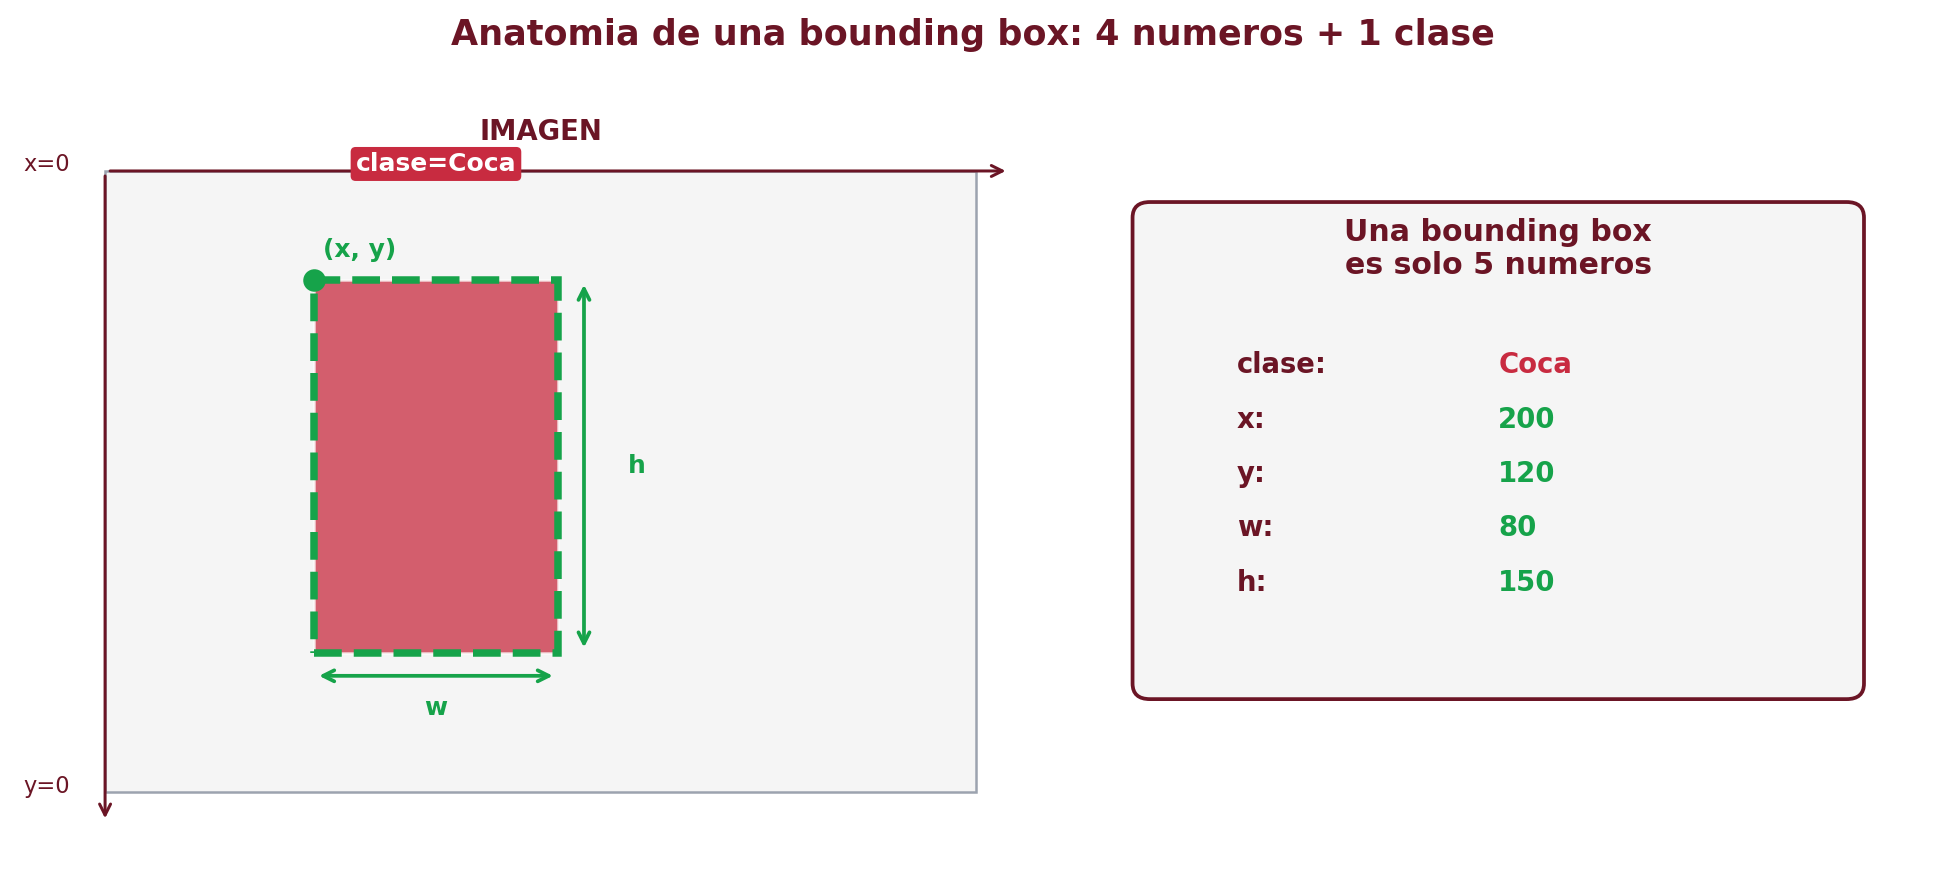
\includegraphics[width=0.95\textwidth]{fig_bbox.png}
  \end{center}

  \vspace{4pt}
  {\scriptsize\color{textMuted}
    \faLightbulb\hspace{4pt} Un bbox = (\textbf{x, y, w, h, clase}).
    Es la unidad b\'asica de la detecci\'on: cada objeto encontrado
    se reporta como un rect\'angulo con su etiqueta.}
\end{frame}

\begin{frame}[shrink]{IoU: ?`Qu\'e Tan Buena Es Una Predicci\'on?}
  \vspace{4pt}
  {\footnotesize\color{arcaDark}\bfseries
    \textbf{IoU} (Intersection over Union) compara la caja real con la
    predicha: $\text{IoU} = \dfrac{\text{intersecci\'on}}{\text{uni\'on}}$. Va de 0 a 1.}

  \vspace{6pt}
  \begin{center}
    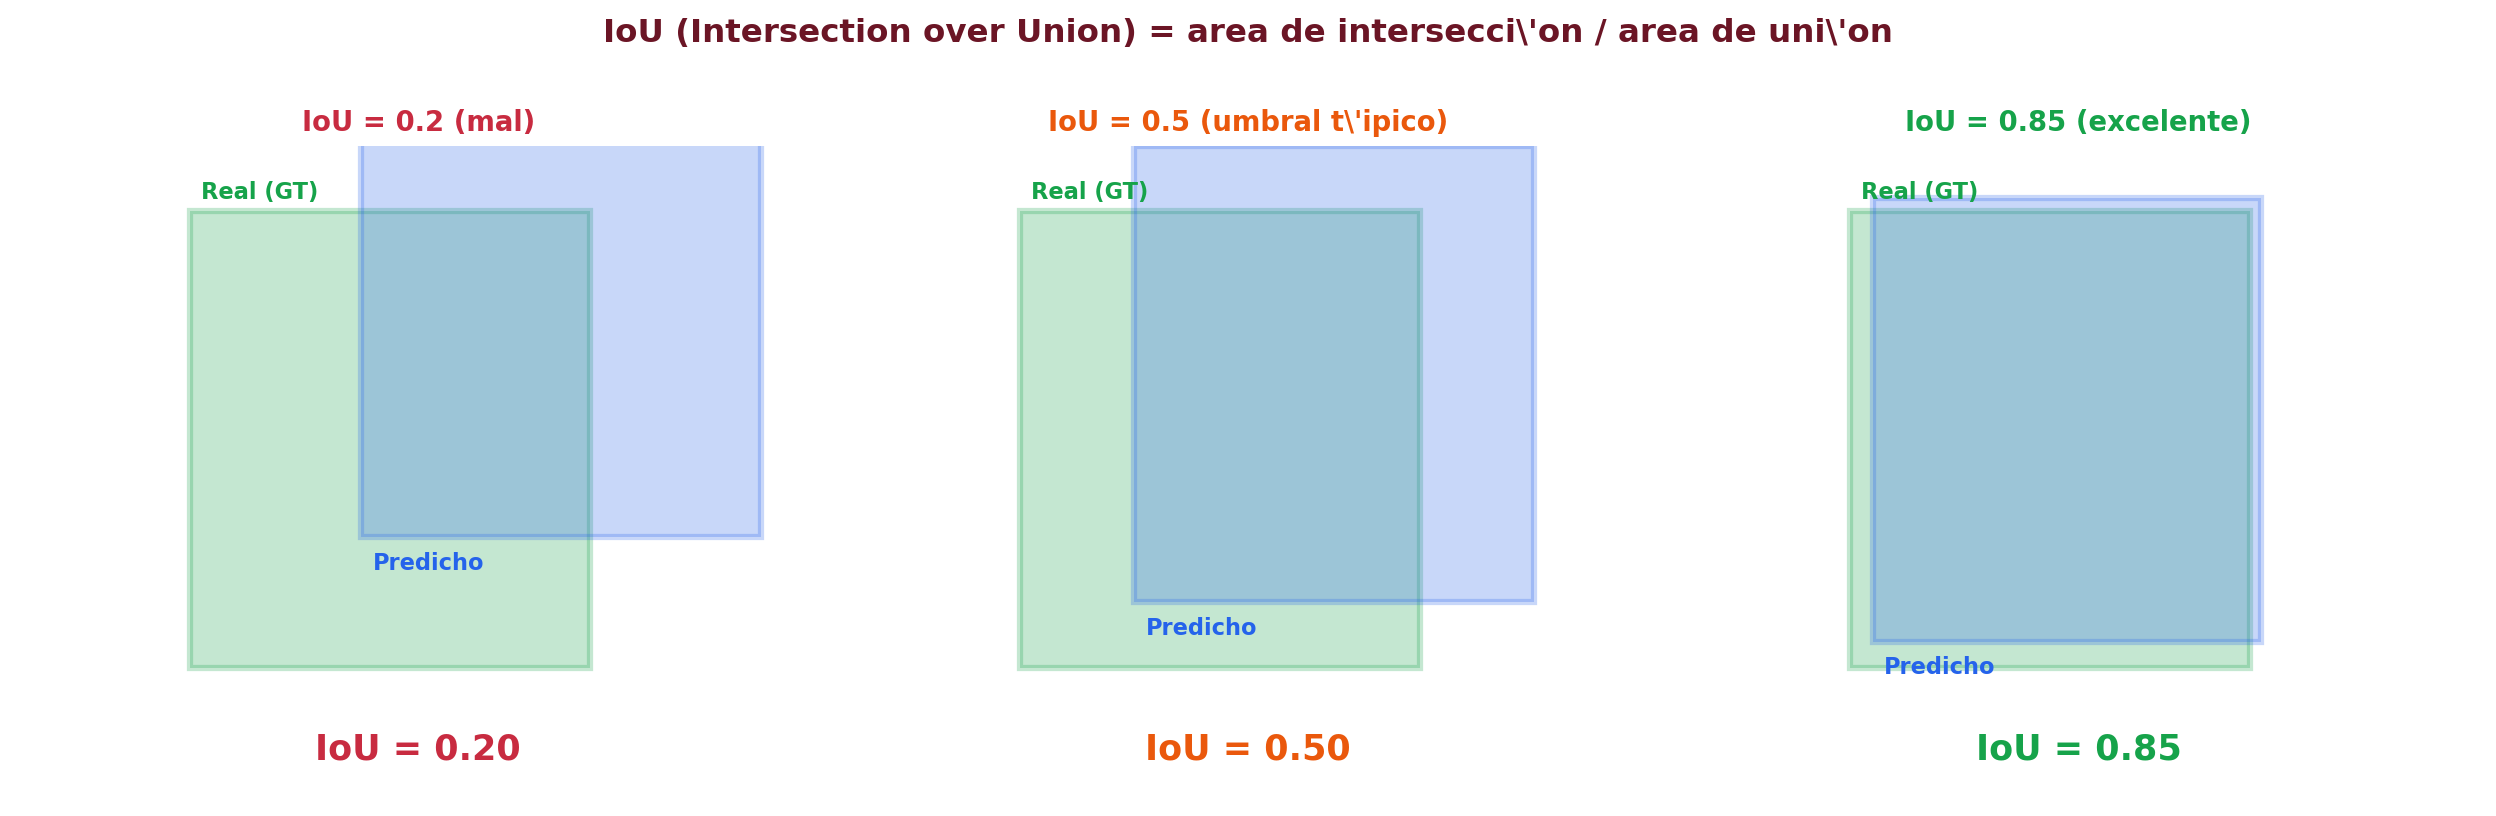
\includegraphics[width=0.95\textwidth]{fig_iou.png}
  \end{center}

  \vspace{2pt}
  {\scriptsize\color{textMuted}
    \faLightbulb\hspace{4pt} Convenci\'on: IoU $\geq$ 0.5 cuenta como
    detecci\'on correcta. Volveremos a esto cuando hablemos de m\'etricas.}
\end{frame}

% =============================================================================
%  BLOQUE F: APP 1 --- SLIDING WINDOW (NUEVO)
% =============================================================================
\sectionframe{App 1: Sliding Window}{?`Y si uso mi CNN para detectar?}

\begin{frame}[shrink]{El Intento Naive: Barrer la Imagen}
  \vspace{6pt}
  {\footnotesize\color{arcaDark}\bfseries
    Tenemos una CNN entrenada en clase 24 que clasifica
    \textbf{Coca vs Pepsi} a nivel de imagen. ?`La podemos usar para
    \emph{detectar} las latas en una foto con varias?}

  \vspace{14pt}
  {\footnotesize
  \begin{enumerate}\setlength{\itemsep}{6pt}
    \item[{\color{arcaRed}\bfseries 1.}]
      Recorremos la imagen con una \textbf{ventana deslizante}
      (varios tama\~nos: 64, 96, 128 px).
    \item[{\color{arcaRed}\bfseries 2.}]
      Por cada parche, le preguntamos a la CNN: ``?`es Coca o Pepsi?''
      Si la confianza pasa un umbral, \textbf{guardamos la caja}.
    \item[{\color{arcaRed}\bfseries 3.}]
      Dibujamos todas las cajas que pasaron el umbral.
    \item[{\color{codeGreen}\bfseries 4.}]
      Lo envolvemos en una \textbf{app de Gradio} para que ustedes
      suban su propia foto.
  \end{enumerate}
  }
\end{frame}

\begin{frame}[fragile,shrink]{El C\'odigo del Detector Casero}
  \vspace{-4pt}
  \begin{pyblock}
def sliding_window_detect(img, modelo, ventana=96, paso=24, umbral=0.85):
    cajas = []
    H, W, _ = img.shape
    for y in range(0, H - ventana, paso):
        for x in range(0, W - ventana, paso):
            parche = img[y:y+ventana, x:x+ventana]
            prob = modelo.predict(parche[None, ...], verbose=0)[0]
            clase = prob.argmax()
            conf  = prob.max()
            if conf > umbral:
                cajas.append((x, y, ventana, ventana, clase, conf))
    return cajas
  \end{pyblock}

  \vspace{4pt}
  {\scriptsize\color{textMuted}
    \faLightbulb\hspace{4pt} En Colab corremos este c\'odigo, lo
    envolvemos con \texttt{gradio.Interface}, y \texttt{share=True}
    nos da un link p\'ublico para que cada uno lo pruebe.}
\end{frame}

\begin{frame}[shrink]{Lo Que Vamos a Ver en Vivo}
  \vspace{6pt}
  {\footnotesize\color{arcaDark}\bfseries
    Suben una foto de una nevera con varias latas y miran la app.
    Esto es lo que va a pasar:}

  \vspace{10pt}
  {\footnotesize
  \begin{itemize}\setlength{\itemsep}{6pt}
    \item[{\color{arcaRed}\scriptsize\faClock}]
      \textbf{Lentitud:} barrer una imagen 600$\times$400 con paso 24
      son $\sim$400 inferencias. La app tarda \textbf{varios segundos}.
    \item[{\color{arcaRed}\scriptsize\faCopy}]
      \textbf{Cajas duplicadas:} cada lata aparece detectada por
      muchas ventanas vecinas. Un mont\'on de rect\'angulos solapados.
    \item[{\color{arcaRed}\scriptsize\faRulerCombined}]
      \textbf{Tama\~no fijo:} la ventana es 96$\times$96. Una lata m\'as
      grande o m\'as peque\~na no se detecta bien.
    \item[{\color{arcaRed}\scriptsize\faQuestionCircle}]
      \textbf{Falsos positivos:} una etiqueta roja en una bolsa no es
      una Coca, pero la CNN dice que s\'i.
  \end{itemize}
  }
\end{frame}

\begin{frame}[shrink]{El Techo de la Clasificaci\'on}
  \vspace{6pt}
  {\footnotesize\color{arcaDark}\bfseries
    Funciona\ldots m\'as o menos. Pero el costo es alto y la calidad
    es pobre. \textbf{No escala}.}

  \vspace{14pt}
  {\footnotesize
  \begin{tabular}{@{}p{4.0cm} p{4.0cm} p{4.0cm}@{}}
    \toprule
    \textbf{Problema} & \textbf{CNN cl\'asica} & \textbf{Lo que necesitamos} \\
    \midrule
    \rowcolor{arcaGray}
    Salida
    & 1 vector fijo
    & Lista variable de bboxes \\
    Cantidad de objetos
    & Asume 1
    & Puede ser 0, 1 o 100 \\
    \rowcolor{arcaGray}
    Ubicaci\'on
    & No la sabe
    & Da (x, y, w, h) por objeto \\
    Velocidad
    & Una pasada por imagen
    & Una pasada total, no 400 \\
    \bottomrule
  \end{tabular}
  }

  \vspace{14pt}
  \begin{tcolorbox}[colback=arcaRed!8, colframe=arcaRed, boxrule=0.5pt,
    arc=2pt, left=6pt, right=6pt, top=4pt, bottom=4pt]
    {\scriptsize\color{arcaDark}
    \faExclamationTriangle\hspace{4pt} Hace falta una arquitectura
    \emph{dise\~nada} para producir m\'ultiples bboxes en una sola
    pasada. Esa es la idea de \textbf{YOLO}.}
  \end{tcolorbox}
\end{frame}

% =============================================================================
%  BLOQUE G: YOLO EN PROFUNDIDAD
% =============================================================================
\sectionframe{C\'omo Funciona YOLO}{La idea revolucionaria de 2015}

\begin{frame}[shrink]{La Idea: ``You Only Look Once''}
  \vspace{6pt}
  {\footnotesize\color{arcaDark}\bfseries
    Antes de YOLO los detectores hac\'ian dos pasadas: primero proponer
    regiones, despu\'es clasificar cada una. \textbf{Lento}.
    YOLO lo hace todo en \textbf{una sola pasada} de la CNN.}

  \vspace{14pt}
  {\footnotesize
  \begin{enumerate}\setlength{\itemsep}{6pt}
    \item[{\color{arcaRed}\bfseries 1.}]
      \textbf{Divide la imagen en una rejilla} (ej: 13$\times$13).
    \item[{\color{arcaRed}\bfseries 2.}]
      Cada celda predice: ``?`hay un objeto centrado en m\'i?'' Si s\'i,
      devuelve una bbox completa (x, y, w, h, clase, confianza).
    \item[{\color{arcaRed}\bfseries 3.}]
      \textbf{Una sola pasada} de la red $\Rightarrow$ todas las cajas a la vez.
    \item[{\color{codeGreen}\bfseries 4.}]
      Al final, \textbf{NMS} limpia las cajas duplicadas.
  \end{enumerate}
  }
\end{frame}

\begin{frame}[shrink]{La Rejilla en la Pr\'actica}
  \vspace{4pt}
  \begin{center}
    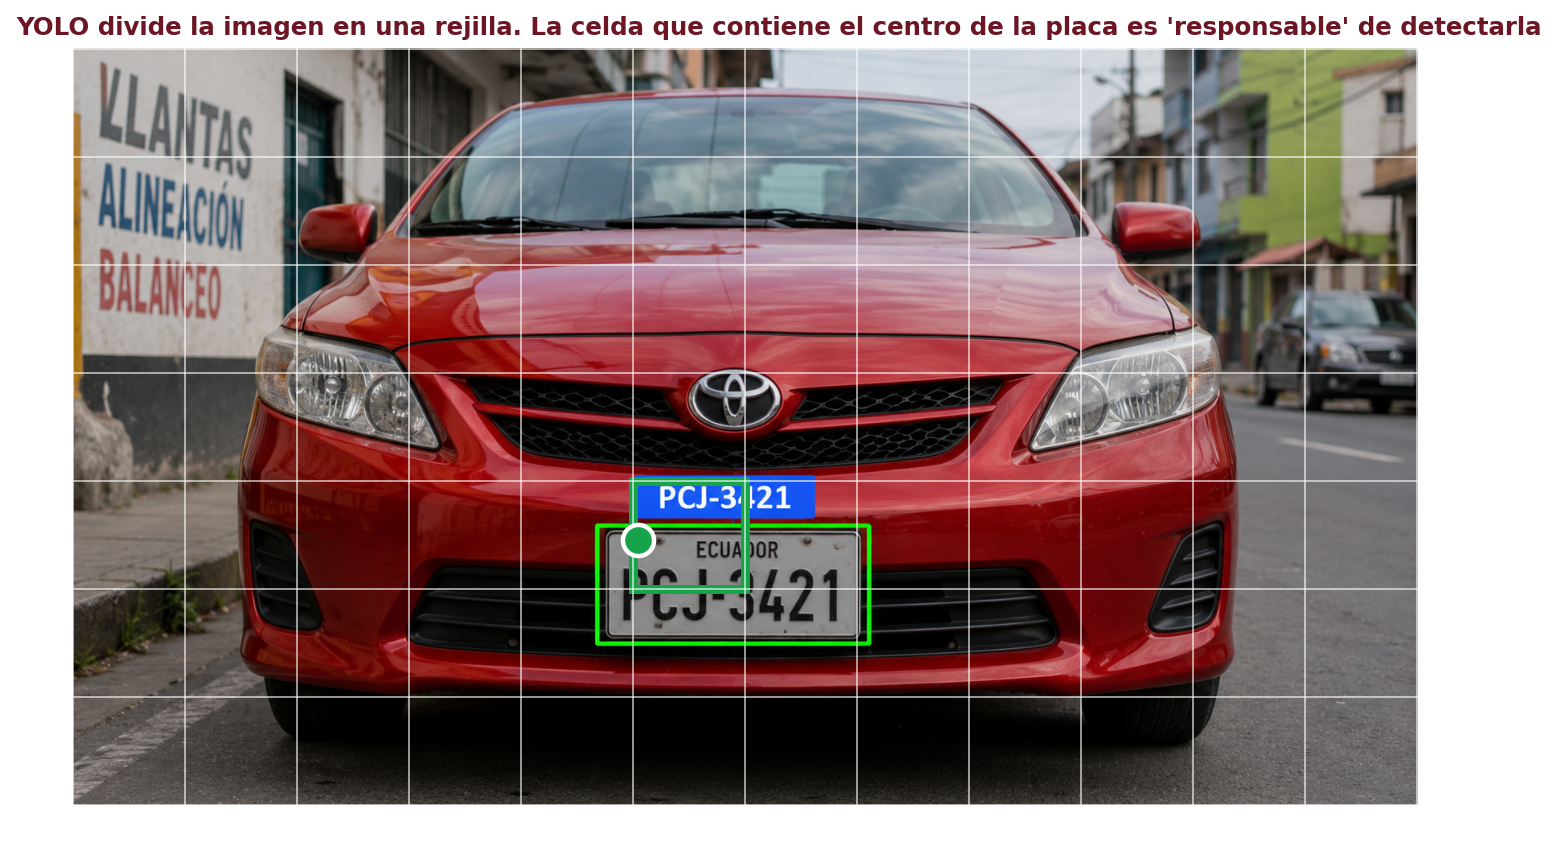
\includegraphics[width=0.85\textwidth]{fig_yolo_grid.png}
  \end{center}

  \vspace{4pt}
  {\scriptsize\color{textMuted}
    \faLightbulb\hspace{4pt} La celda donde cae el centro del objeto
    es \emph{responsable} de detectarlo.
    En YOLO26 hay 3 escalas de rejilla simult\'aneas
    para detectar objetos de distintos tama\~nos.}
\end{frame}

\begin{frame}[shrink]{NMS: Limpiar Detecciones Duplicadas}
  \vspace{4pt}
  {\footnotesize\color{arcaDark}\bfseries
    YOLO produce \textbf{cientos} de detecciones por imagen, varias
    del mismo objeto. \textbf{NMS} (Non-Maximum Suppression) deja una sola.}

  \vspace{6pt}
  \begin{center}
    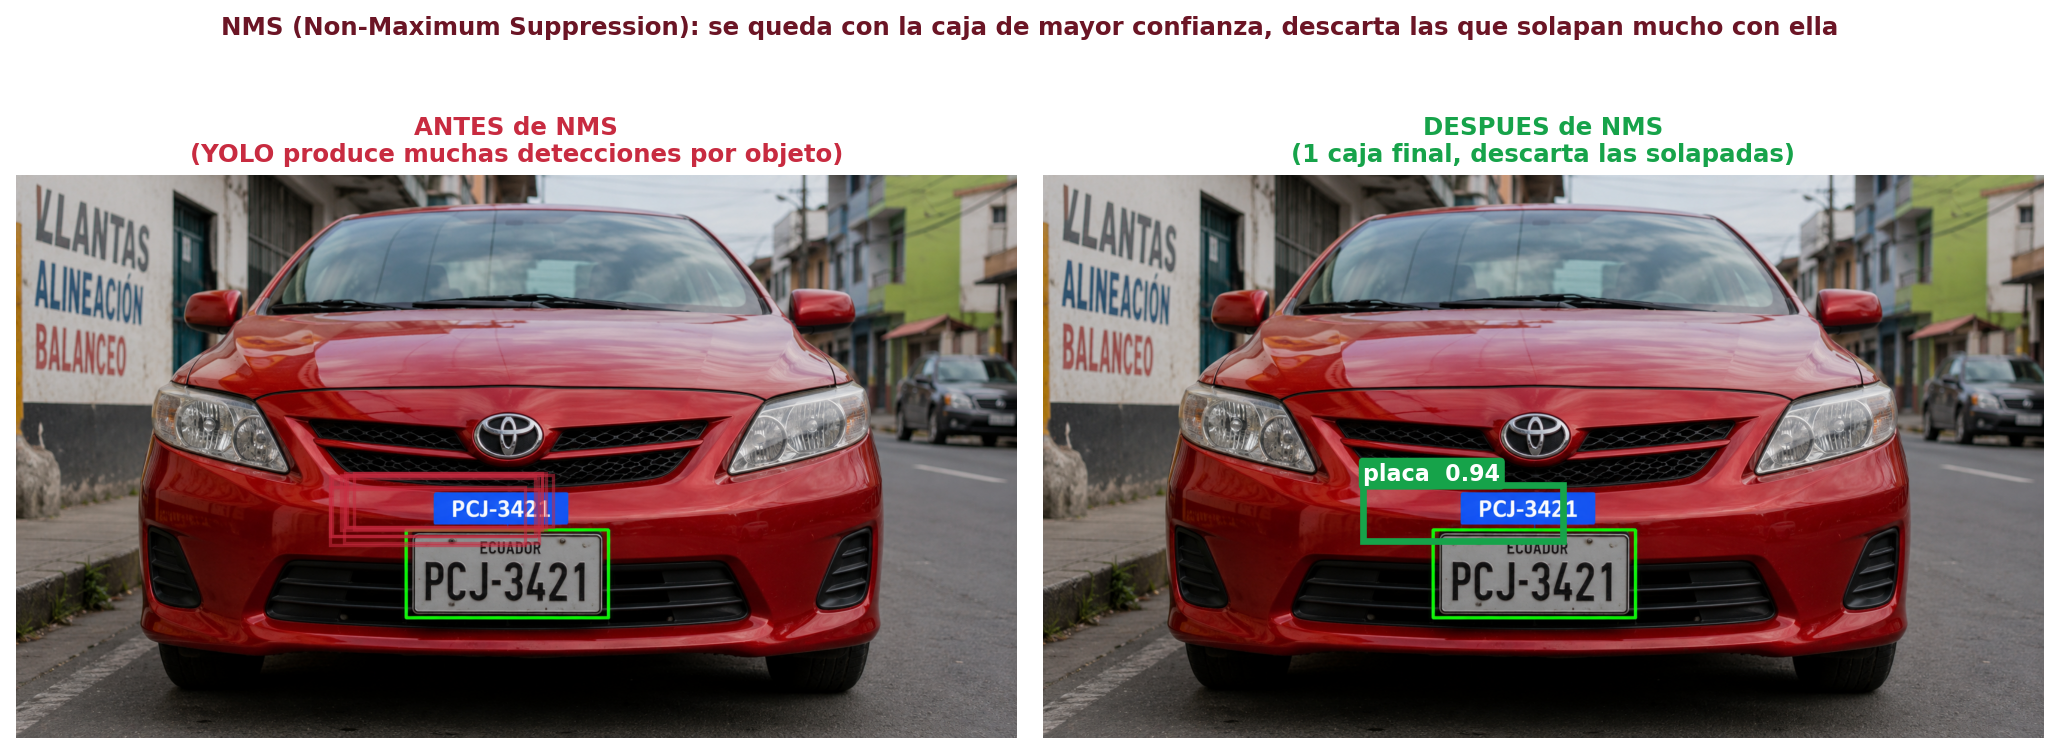
\includegraphics[width=0.95\textwidth]{fig_nms.png}
  \end{center}

  \vspace{2pt}
  {\scriptsize\color{textMuted}
    \faLightbulb\hspace{4pt} Algoritmo: ordenar por confianza, quedarse
    con la mejor, descartar las que solapan con IoU $>$ 0.5. Repetir.
    Lo mismo que el sliding window deber\'ia haber hecho.}
\end{frame}

\begin{frame}[shrink]{Una D\'ecada de YOLO}
  \vspace{4pt}
  \begin{center}
    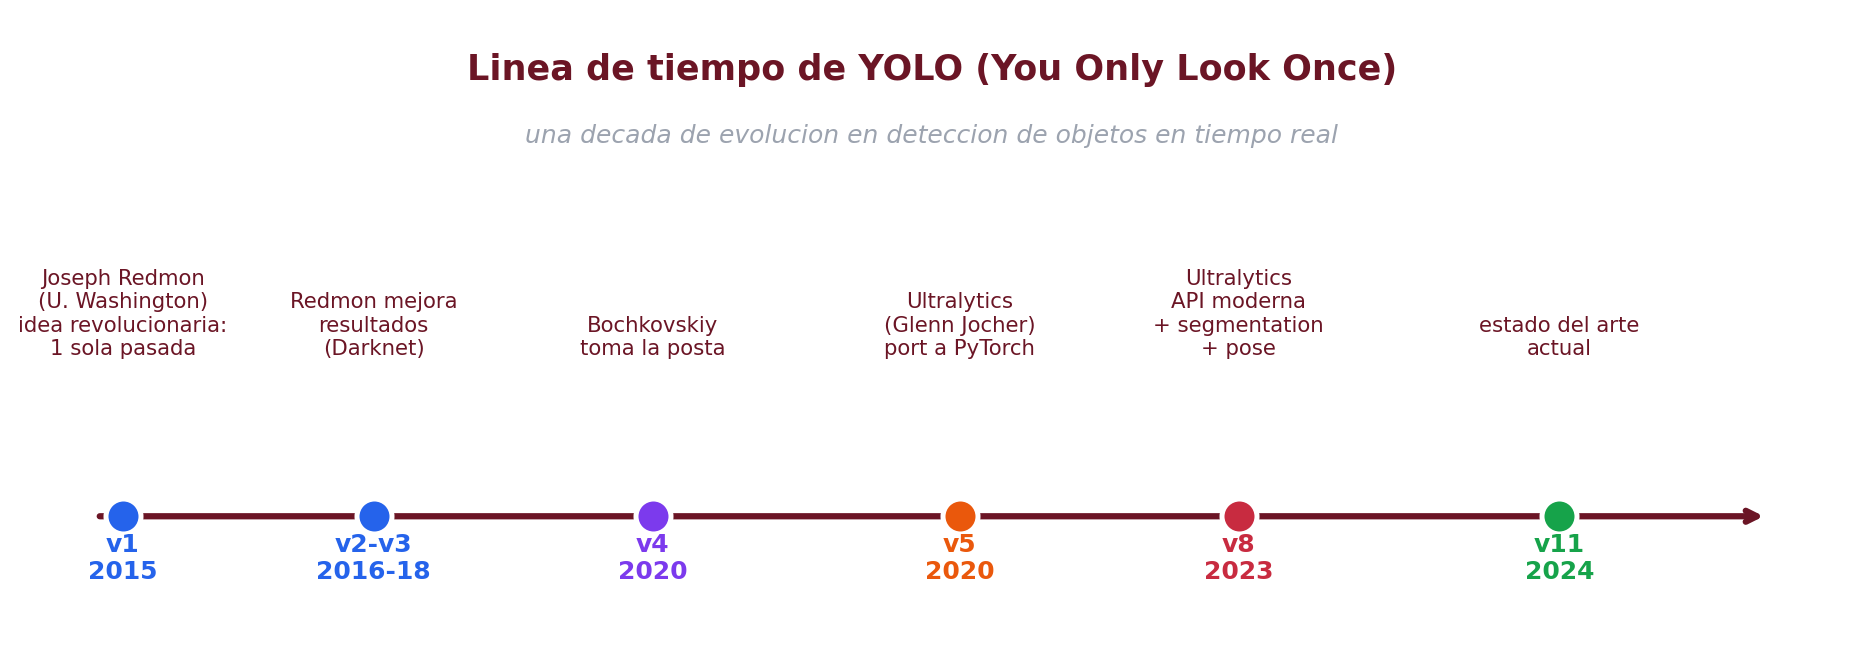
\includegraphics[width=0.97\textwidth]{fig_yolo_timeline.png}
  \end{center}

  \vspace{6pt}
  {\scriptsize
  \begin{itemize}\setlength{\itemsep}{2pt}
    \item[{\color{arcaRed}\scriptsize\faArrowRight}]
      \textbf{Joseph Redmon (v1, 2015):} idea original, paper famoso.
      Framework Darknet en C.
    \item[{\color{arcaRed}\scriptsize\faArrowRight}]
      \textbf{Bochkovskiy (v4, 2020):} continu\'o cuando Redmon abandon\'o.
    \item[{\color{arcaRed}\scriptsize\faArrowRight}]
      \textbf{Ultralytics (v5+, 2020+):} port a PyTorch, API moderna.
    \item[{\color{codeGreen}\scriptsize\faArrowRight}]
      \textbf{YOLO26 (Ultralytics, ene 2026):} \'ultima versi\'on,
      es la que vamos a usar.
  \end{itemize}
  }
\end{frame}

\begin{frame}[shrink]{La Familia: Velocidad vs Precisi\'on}
  \vspace{4pt}
  \begin{center}
    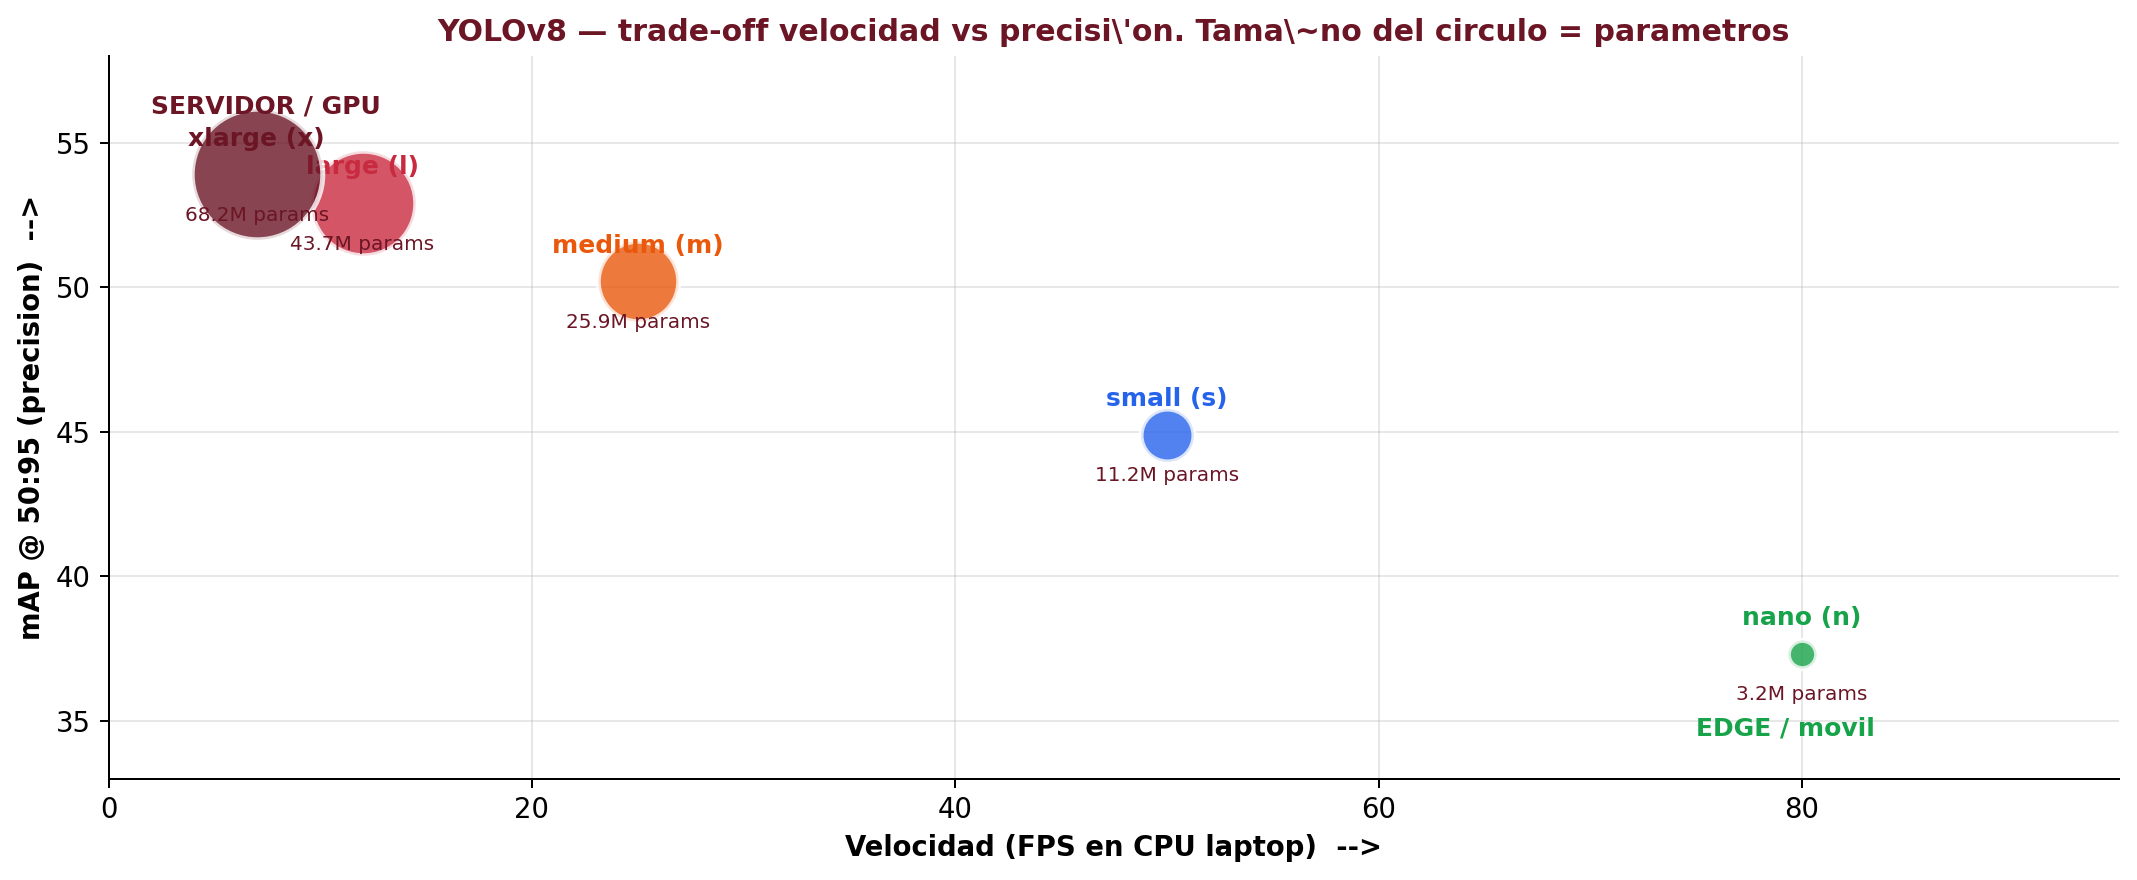
\includegraphics[width=0.92\textwidth]{fig_yolo_family.png}
  \end{center}

  \vspace{4pt}
  {\scriptsize\color{textMuted}
    \faLightbulb\hspace{4pt} 5 tama\~nos (n, s, m, l, x): la \emph{misma}
    arquitectura con distinta cantidad de filtros. M\'as filtros = m\'as
    preciso pero m\'as lento.}
\end{frame}

\begin{frame}[shrink]{?`Cu\'al Modelo Eligir?}
  \vspace{8pt}
  {\footnotesize
  \begin{tabular}{@{}p{2.0cm} p{3.7cm} p{2.7cm} p{4.0cm}@{}}
    \toprule
    \textbf{Modelo} & \textbf{Hardware} & \textbf{Velocidad} & \textbf{Cu\'ando usarlo} \\
    \midrule
    \rowcolor{arcaGray}
    \textbf{nano (n)}  & CPU laptop, m\'ovil & 80+ FPS & Edge, IoT, c\'amara en vivo \\
    small (s)  & CPU buena o GPU peque\~na & 50 FPS & Demo r\'apido, prototipo \\
    \rowcolor{arcaGray}
    medium (m) & GPU consumer & 25 FPS & Producci\'on con buen hardware \\
    large (l)  & GPU dedicada & 12 FPS & Calidad alta, no tiempo real \\
    \rowcolor{arcaGray}
    xlarge (x) & GPU servidor & 7 FPS & M\'axima precisi\'on, batch off-line \\
    \bottomrule
  \end{tabular}
  }

  \vspace{14pt}
  \begin{tcolorbox}[colback=codeGreen!8, colframe=codeGreen, boxrule=0.5pt,
    arc=2pt, left=6pt, right=6pt, top=4pt, bottom=4pt]
    {\scriptsize\color{arcaDark}
    \faKey\hspace{4pt} Para nuestras pruebas y proyecto vamos con
    \textbf{YOLO26 nano}. Funciona en CPU de Colab y carga en segundos.}
  \end{tcolorbox}
\end{frame}

% =============================================================================
%  BLOQUE H: PROYECTO LPR + APP 2 YOLO PREENTRENADO
% =============================================================================
\sectionframe{App 2: YOLO en Vivo}{?`Nos sirve preentrenado para nuestro problema?}

\begin{frame}[shrink]{El Proyecto que Viene: Lectura de Placas}
  \vspace{6pt}
  {\footnotesize\color{arcaDark}\bfseries
    Imaginen este caso real de Arca: control de acceso a planta.
    Cada cami\'on que entra debe registrarse en un libro --- un guardia
    anota la placa con bol\'igrafo. Lento, propenso a errores.}

  \vspace{6pt}
  \begin{center}
    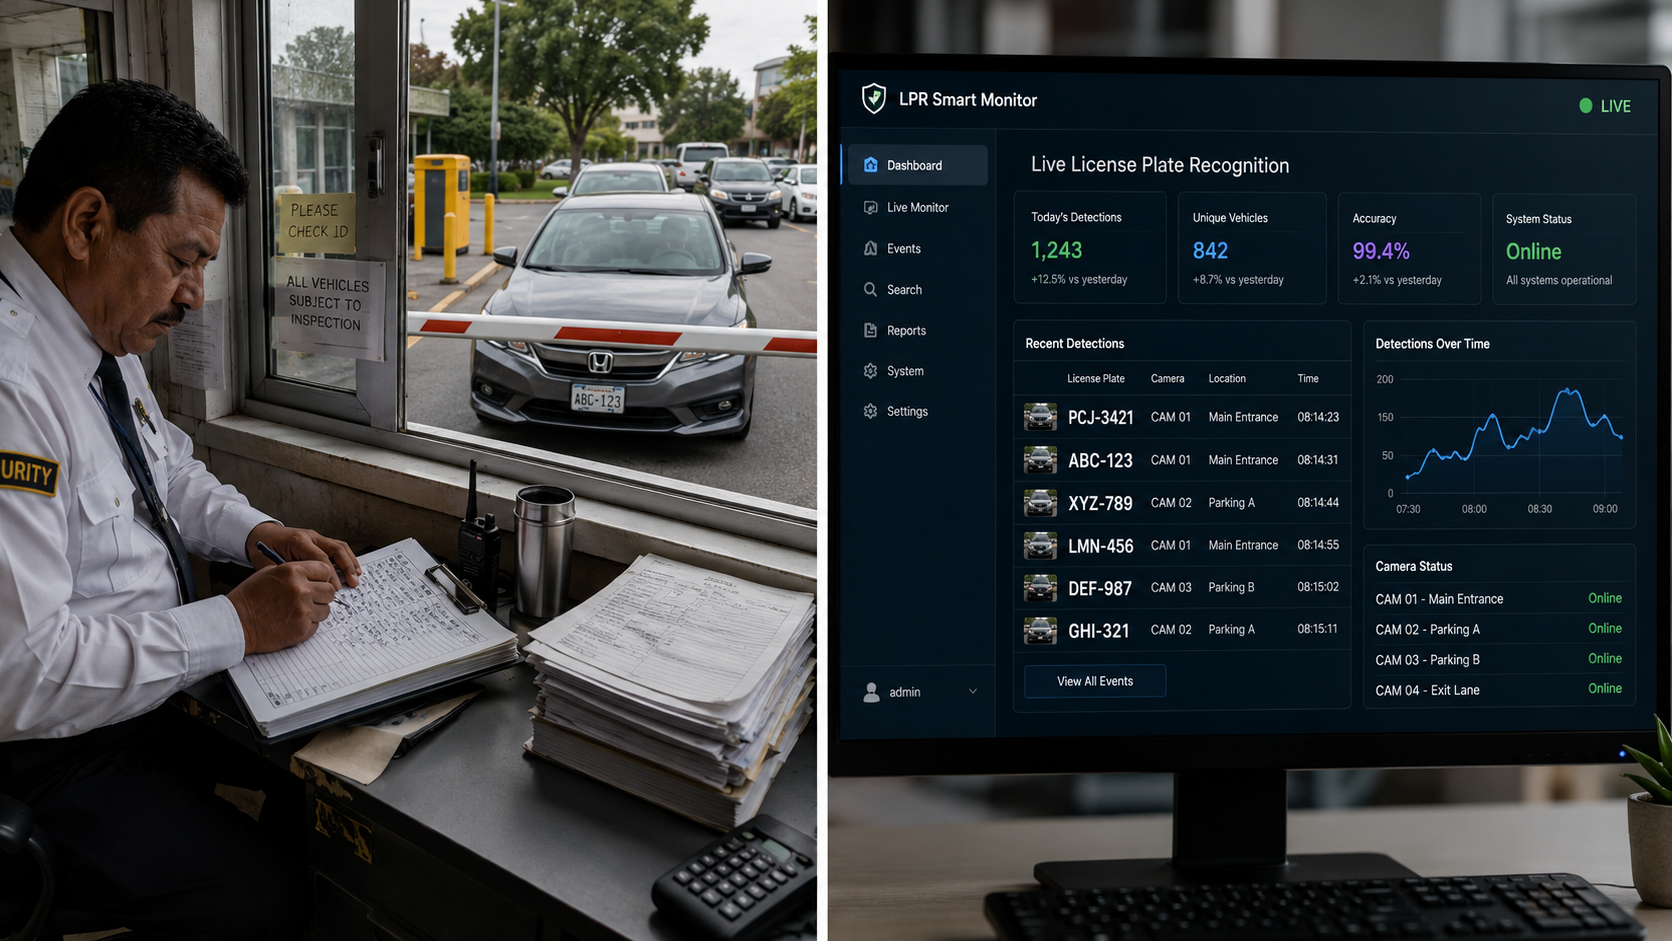
\includegraphics[width=0.55\textwidth]{fig_motivacion_problema.png}
  \end{center}

  \vspace{2pt}
  {\scriptsize\color{textMuted}
    \faLightbulb\hspace{4pt} \textbf{Lo que vamos a construir las pr\'oximas
    clases:} una app que recibe foto de un veh\'iculo y devuelve la placa
    le\'ida en texto, autom\'aticamente.}
\end{frame}

\begin{frame}[fragile,shrink]{YOLO en 4 L\'ineas}
  \vspace{-4pt}
  \begin{pyblock}
from ultralytics import YOLO
modelo = YOLO("yolo26n.pt")           # se descarga la primera vez

resultado = modelo.predict("foto.jpg", conf=0.25)
resultado[0].show()                   # dibuja las cajas detectadas
  \end{pyblock}

  \vspace{4pt}
  {\scriptsize\color{textMuted}
    \faLightbulb\hspace{4pt} El modelo viene preentrenado en
    \textbf{COCO}: 80 clases comunes (persona, carro, perro, botella,
    etc.). Sin entrenar nada, ya detecta esas 80 clases.}
\end{frame}

\begin{frame}[shrink]{La App de Gradio en Colab}
  \vspace{6pt}
  {\footnotesize\color{arcaDark}\bfseries
    Vamos al Colab y montamos una app sencilla:
    suben una foto $\to$ YOLO la procesa $\to$ ven las cajas y las clases.}

  \vspace{12pt}
  {\footnotesize
  \begin{enumerate}\setlength{\itemsep}{6pt}
    \item[{\color{arcaRed}\bfseries 1.}]
      Cargar \texttt{yolo26n.pt} (nano, $\sim$6 MB).
    \item[{\color{arcaRed}\bfseries 2.}]
      Funci\'on \texttt{detectar(img)} que llama a \texttt{modelo.predict}
      y devuelve la imagen anotada.
    \item[{\color{arcaRed}\bfseries 3.}]
      \texttt{gradio.Interface} con input imagen + output imagen.
    \item[{\color{codeGreen}\bfseries 4.}]
      \texttt{share=True} $\to$ link p\'ublico, todos pueden subir su foto.
  \end{enumerate}
  }
\end{frame}

\begin{frame}[shrink]{Experimento 1: Suban Una Foto Cualquiera}
  \vspace{6pt}
  {\footnotesize\color{arcaDark}\bfseries
    Foto de la oficina, de una calle, de la planta, de su gato, de
    una nevera con producto. Cualquier cosa. Miren qu\'e detecta.}

  \vspace{14pt}
  {\footnotesize
  \begin{itemize}\setlength{\itemsep}{6pt}
    \item[{\color{codeGreen}\scriptsize\faCheck}]
      \textbf{Personas, carros, perros, sillas, botellas:} las detecta
      al instante con confianza alta.
    \item[{\color{codeGreen}\scriptsize\faCheck}]
      \textbf{Una sola pasada:} milisegundos por foto, no segundos.
    \item[{\color{codeGreen}\scriptsize\faCheck}]
      \textbf{Sin cajas duplicadas:} NMS ya se encarga.
    \item[{\color{codeGreen}\scriptsize\faCheck}]
      \textbf{M\'ultiples objetos:} 5 personas en la foto, 5 cajas con etiqueta correcta.
  \end{itemize}
  }

  \vspace{8pt}
  \begin{tcolorbox}[colback=codeGreen!8, colframe=codeGreen, boxrule=0.5pt,
    arc=2pt, left=6pt, right=6pt, top=4pt, bottom=4pt]
    {\scriptsize\color{arcaDark}
    \faKey\hspace{4pt} Qued\'o claro el salto vs sliding window.}
  \end{tcolorbox}
\end{frame}

\begin{frame}[shrink]{Experimento 2: Ahora Suban Una Placa}
  \vspace{6pt}
  {\footnotesize\color{arcaDark}\bfseries
    Suban una foto de un carro --- de la calle, de su celular,
    una de las del repo. Miren qu\'e detecta YOLO.}

  \vspace{14pt}
  {\footnotesize
  \begin{itemize}\setlength{\itemsep}{6pt}
    \item[{\color{codeGreen}\scriptsize\faCheck}]
      Detecta \texttt{car} con alta confianza.
    \item[{\color{codeGreen}\scriptsize\faCheck}]
      A veces detecta \texttt{truck}, \texttt{person} (conductor), \texttt{wheel}.
    \item[{\color{arcaRed}\scriptsize\faTimes}]
      \textbf{Pero NO detecta la placa.} Ni siquiera la dibuja.
    \item[{\color{arcaRed}\scriptsize\faTimes}]
      No es un bug. Es que \textbf{``placa'' no est\'a entre las 80 clases de COCO}.
      YOLO nunca vio una placa etiquetada como tal.
  \end{itemize}
  }
\end{frame}

\begin{frame}[shrink]{La Conclusi\'on}
  \vspace{8pt}
  {\footnotesize\color{arcaDark}\bfseries
    YOLO preentrenado es brutal --- pero solo ve lo que le ense\~naron.
    Para nuestro problema necesitamos \textbf{ense\~narle a ver placas}.}

  \vspace{14pt}
  {\footnotesize
  \begin{itemize}\setlength{\itemsep}{6pt}
    \item[{\color{arcaRed}\scriptsize\faArrowRight}]
      Esto es el mismo movimiento que clase 24:
      \textbf{transfer learning + fine-tuning}.
    \item[{\color{arcaRed}\scriptsize\faArrowRight}]
      Tomamos YOLO26n preentrenado en COCO (sabe ver bordes,
      texturas, formas, objetos) y le agregamos una clase nueva: \texttt{placa}.
    \item[{\color{arcaRed}\scriptsize\faArrowRight}]
      Para eso necesitamos \emph{nuestro propio dataset etiquetado}
      con bboxes de placas. (?`Recuerdan las 5 reglas de oro?)
    \item[{\color{codeGreen}\scriptsize\faArrowRight}]
      Eso es lo que viene en las pr\'oximas clases.
  \end{itemize}
  }
\end{frame}

% =============================================================================
%  CIERRE
% =============================================================================
\sectionframe{Cierre}{Lo que aprendimos hoy}

\begin{frame}[shrink]{Resumen}
  \vspace{6pt}
  \begin{columns}[T]
    \begin{column}{0.48\textwidth}
      {\footnotesize\bfseries\color{arcaDark} Clasificaci\'on a fondo:}
      \vspace{4pt}

      {\scriptsize
      Transfer learning con VGG16, costos reales de las CNN, c\'omo
      armar un dataset bueno (5 reglas de oro, errores comunes).

      \vspace{8pt}
      \textbf{El techo:}

      \vspace{4pt}
      Sliding window con la CNN cl\'asica funciona\ldots m\'as o menos.
      Lento, cajas duplicadas, no escala.
      }
    \end{column}
    \begin{column}{0.48\textwidth}
      {\footnotesize\bfseries\color{arcaDark} Detecci\'on:}
      \vspace{4pt}

      {\scriptsize
      Una bbox = (x, y, w, h, clase). Calidad medida con IoU.
      \textbf{YOLO}: una sola pasada, rejilla, NMS.

      \vspace{8pt}
      \textbf{La pregunta abierta:}

      \vspace{4pt}
      YOLO preentrenado no ve placas. ?`C\'omo le ense\~namos?
      }
    \end{column}
  \end{columns}

  \vspace{12pt}
  \begin{tcolorbox}[colback=codeGreen!8, colframe=codeGreen, boxrule=0.5pt,
    arc=2pt, left=6pt, right=6pt, top=4pt, bottom=4pt]
    {\scriptsize\color{arcaDark}
    \faKey\hspace{4pt}\textbf{Pr\'oxima clase:} m\'etricas de detecci\'on
    (mAP), etiquetar nuestro propio dataset de placas, fine-tunear
    YOLO26 y desplegar.}
  \end{tcolorbox}
\end{frame}

% ── QR DE CIERRE ──────────────────────────────────────────────────────
{
\setbeamertemplate{headline}{}
\setbeamertemplate{footline}{}
\begin{frame}[plain, noframenumbering]
  \begin{tikzpicture}[remember picture, overlay]
    \fill[arcaDark] (current page.south west) rectangle (current page.north east);
  \end{tikzpicture}
  \vspace{1.0cm}
  \begin{center}
    {\color{white}\Huge\bfseries Encuesta de Cierre} \\[0.4cm]
    {\color{white!85}\Large Cu\'entanos qu\'e tal estuvo la clase}
    \vspace{1cm}

    
\includegraphics[width=4.5cm]{qr_encuesta.jpg}

    \vspace{0.6cm}
    {\color{white!80}\small Gracias por hoy --- nos vemos el lunes}
  \end{center}
\end{frame}
}

\end{document}
